\documentclass{template/tp}
\usepackage[utf8x]{inputenc}

\usepackage[frenchb]{babel}
\usepackage[T1]{fontenc}

\usepackage{graphicx}
\usepackage{amssymb}
\usepackage{amsmath}
\usepackage{wasysym} %smiley
\usepackage{mathastext} % math as standfard text : units are respecting typography conventions.
\usepackage{hyperref}% hyperliens
\usepackage{tikz}
\usetikzlibrary{babel,calc,angles,positioning,intersections,quotes,decorations.markings}
\usepackage{tkz-euclide}
\usetkzobj{all}
\usepackage[]{circuitikz}
\usepackage{textcomp}
\usepackage{minted}
\usepackage[long]{datetime}
\usepackage{gensymb} % \ohm, celsius
\usepackage{framed}
\usepackage{pdfpages}
\usepackage{todo}
\usepackage{paralist}
\usepackage{multicol}
\usepackage{expl3}
\usepackage{xfrac}
\ExplSyntaxOn
\cs_set_eq:NN \fpeval \fp_eval:n
\ExplSyntaxOff



\usepackage{fancyhdr} %en-tête
\usepackage{qrcode}

% \langexam{frenchb}


\newboolean{koriG}
\ifx\koriG\undefined
\correction{false}
\else
\correction{true}
\fi

\author{Renaud Theunissen, Youssef Agram}

%Corrigé ou non?
%\correction{true}
\correction{false}

% Quel TP en pdf output?
%%% fancy header & foot
\pagestyle{fancy}
\lhead{[ELEC-H-2001] Électricité\\ LABO \no 1A : Circuits réactifs en régime - Phaseurs et impédances \ifthenelse{\boolean{corrige}}{~-- corrigé}{}}
\rhead{v1.0.0\\ page \thepage}
\cfoot{}
%%

\pdfinfo{
/Author (Renaud Theunissen et Youssef Agram, ULB -- BEAMS-EE)
/Title (Laboratoire 1A ELEC-H-2001, Circuits réactifs en régime - Phaseurs et impédances)
/ModDate (D:\pdfdate)
}

\hypersetup{
pdftitle={Labo 1A [ELEC-H-2001] Électricité : LABO 1A ELEC-H-2001, Circuits réactifs en régime - Phaseurs et impédances},
pdfauthor={Renaud Theunissen et Youssef Agram, ©2020 ULB - BEAMS-EE},
}

\setlength{\parskip}{0.5cm plus4mm minus3mm} %espacement entre §
\setlength{\parindent}{0pt}


\begin{document}

\tptitle{}{Séance 1A~: Circuits réactifs en régime - Phaseurs et impédances}
\section{But de la manipulation}
Le but de cette séance est de vous familiariser avec le matériel de laboratoire et de vous amener à développer une approche d'investigation des phénomènes liés aux circuits électriques étudiés dans le cours d'ELEC-H-2001.

Pour ce laboratoire vous aurez besoin des éléments suivants :
\begin{itemize}
    \item Votre PicoScope
    \item Les trois sondes (câbles BNC fournis dans le kit).
    \item Le protoboard
    \item Les résistances $R_e$, $R_i$ et $R_j$
    \item L'inductance $L$
    \item Le condensateur $C_i$
\end{itemize}

\section{Pré-requis}
Pour réaliser cette séance de laboratoire, il vous est recommandé de relire attentivement les sections du syllabus suivantes :
\begin{itemize}
    \item Section 4.3 - Adaptation d'impédance
    \item Sections 5.1 à 5.3 - Loi des mailles et utilisation
    \item Section 7.3 - Phaseurs
    \item Section 7.4 - Impédances et admittances
\end{itemize}

\newpage

\section{Préliminaire théorique}
Soit le circuit ci-dessous où $R_1 = 20k\Omega$, $R_2 = 30k\Omega$ et $R_3 = 50k\Omega$:
\begin{center}
\begin{figure}[h!]
    \centering
    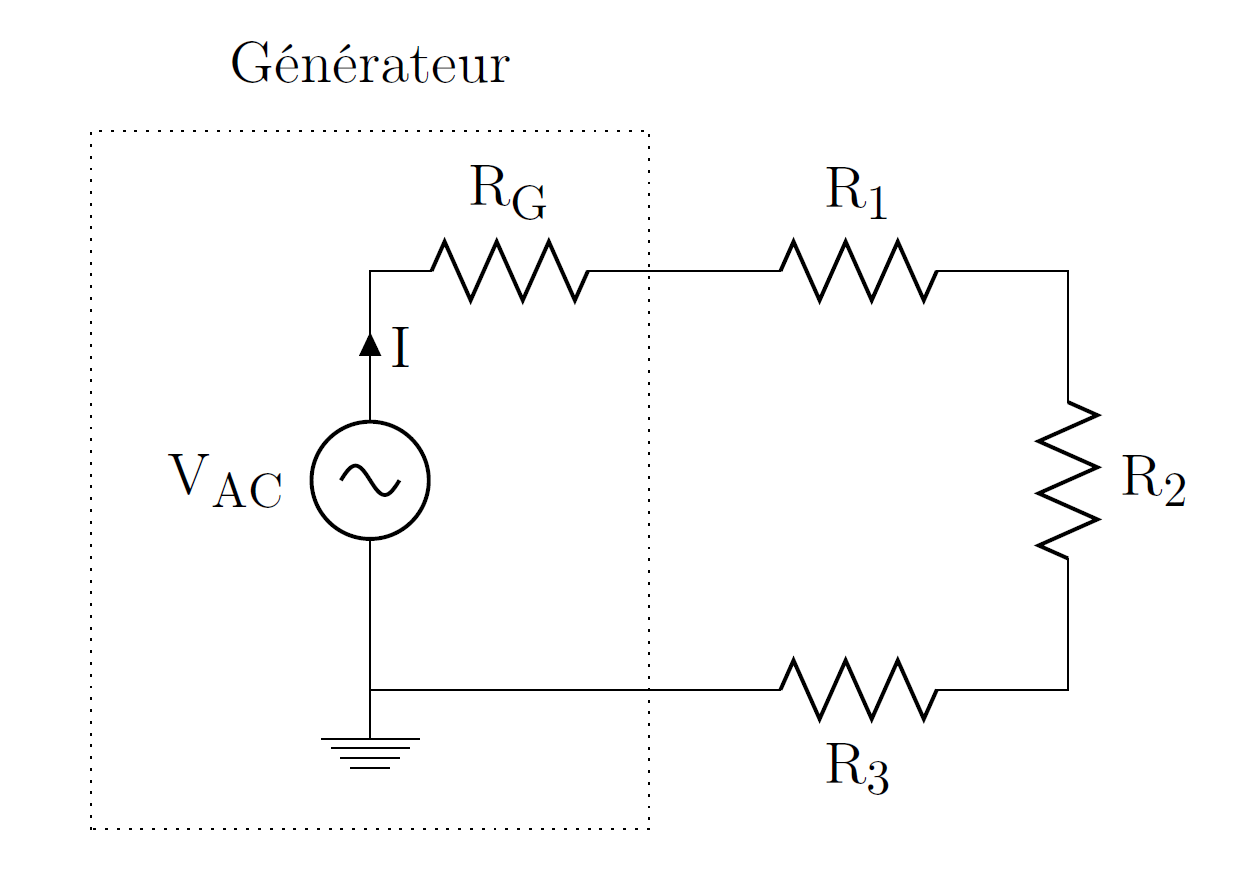
\includegraphics[scale = 0.7]{LABO1A/Ex1Lab1A.PNG}
    \caption{Circuit résistif}
    \label{fig:my_label}
\end{figure}
\end{center}
Si on impose une source $V_{AC}(t) = 10\sqrt{2} cos(2\pi 100t)$, on mesure à l'ampèremètre un courant efficace $I_{eff} = 0,1 mA$.

\subsection{Exercice 1}
\Question
{
\textit{Dans ce circuit, l'impédance de sortie $R_G$ du générateur peut-elle être négligée? Justifiez.}
}
{On observe dans la datasheet du Picoscope\footnote{https://www.picotech.com/oscilloscope/2000/picoscope-2000-manuals} que la résistance de sortie est de $600\Omega$.\\$R_G\ll R_{eq}=R_G+R_1+R_2+R_3=0.6+20+30+50=100.6 k\Omega$, donc $R_G\simeq 0.6\%R_{eq}$.\\
En réalité, la tension en sortie du générateur est donc de $10-0.6*0.1=9.94\ V$. Ceci n'est pas vraiment négligeable donc il est important d'en être conscient. Les résistances utilisées seront de même ordre de grandeur que celle de sortie du générateur. Il faudra donc le prendre en compte.}
\subsection{Exercice 2}
\Question
{
\textit{Vérifiez algébriquement la loi des mailles de ce circuit dans le domaine temporel.}}
{$$v_{AC}(t)=v_1(t)+v_2(t)+v_3(t)$$
$$\iff V_{AC_{eff}}\sqrt{2}\cos(2\pi100t)=(R_1+R_2+R_3)I_{eff}\sqrt{2}\cos(2\pi100t)$$
$$ \iff V_{AC_{eff}}=(R_1+R_2+R_3)I_{eff}=(20+30+50)\times 0.1 \longrightarrow OK$$}
\subsection{Exercice 3}
\Question
{\textit{Vérifiez la loi des mailles géométriquement dans le plan des phaseurs.}}
{La loi des mailles en phaseurs peut s'écrire $\underline{V_{AC}}=(R_1+R_2+R_3)\underline{I}$. Le circuit étant purement résistif, tous les signaux ont une phase nulle.
\begin{figure}[h!]
    \centering
    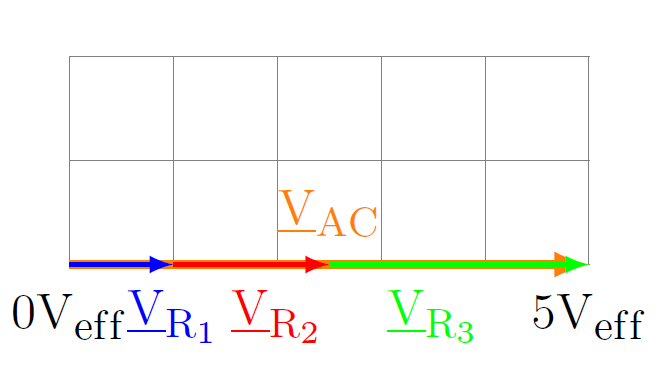
\includegraphics[scale=0.3]{LABO1A/plan_phaseur.PNG}
    \caption{Résolution dans le plan des phaseurs.}
    \label{fig:plan_phaseur}
\end{figure}}
\newpage
\section{Partie pratique}
\subsection{Réflexion analytique et physique}
Notre PicoScope dispose d'une résistance de sortie $R_G$. Si cette résistance est trop importante nous risquons d'avoir une réduction drastique de la tension du générateur.
\Question{
\begin{enumerate}
    \item Comment feriez-vous pour estimer la valeur de cette résistance de sortie ?\\
    \textcolor{darkblue}{L'idée est de connecter le générateur à une charge de résistance connue $R_e$. Ainsi, on pourra calculer la résistance $R_G$ à l'aide de la formule du diviseur résistif: $\underline{V_{AC}}=\frac{R_e}{R_e+R_G}\underline{V_{out}}$}
    \item Donnez la formule d'adaptation d'impédance (en phaseurs) en tension dans le cas où nous aurions un circuit du type :
    \begin{center}
        \begin{circuitikz}\draw
    (0,0)   to[sinusoidal voltage source, v=$v_G(t)$, i^>=$i_G(t)$] 
    (0,4)   to[resistor, l=$R_G$] 
    (4,4)   to[generic, l_=$Z_{charge}$, v^<=$v_{charge}(t)$]
    (4,0)--(0,0)   node[ground]{}
    ;
    \end{circuitikz}
    \end{center}\\
    \vspace{0.5cm}
\textcolor{darkblue}{Nous sommes en présence d'un diviseur résistif: $\underline{V_{G}}=\frac{R_G}{Z_{charge}+R_G}\underline{V_{charge}}$. $R_G$ doit donc être la plus faible possible afin de transmettre au mieux la tension à la charge.}
    \item Dans le cas où $Z_{charge}$ serait une résistance, que devrait valoir cette dernière pour que le module de $v_{charge}(t)$ soit égal à la moitié du module de $v_G(t)$?\\
    \textcolor{darkblue}{Elle devrait être égale à $R_G$}
\end{enumerate}}
{%C
}

\subsection{Mesures de signaux et interprétation - circuit résistif}
Réalisez sur votre \textit{Protoboard} le circuit suivant:
\begin{center}
    \begin{circuitikz} \draw
        (0,0) to[square voltage source, v=$v_{G}(t)$, i^>=$i(t)$] 
        (0,4) --
        (4,4) to[resistor, l_=$R_{i,j}$, v^<=$v_{R_{i,j}}$] 
        (4,0) to[resistor, l=$R_e$]
        (0,0) node[ground] {}
        ;
    \end{circuitikz}
\end{center}
\Question
{
Sachant que :
\begin{itemize}
    \item $R_e = 200\Omega$ 
    \item $v_G(t) = 2V$ et est une onde carrée de fréquence très basse ($f \approx 10Hz$)
    \item $R_G = 600\Omega$
    \item $R_{i,j}$ représente soit la résistance $R_i$ soit la résistance $R_j$ (il faudra tester les deux).
\end{itemize}
déterminez la valeur des résistances $R_i$ et $R_j$. \\
Vérifiez qu'en mettant les deux résistances $R_e$ en série avec les résistances $R_i$ et $R_j$ (donc pour obtenir une résistance équivalente $R_{tot}=R_e+R_e+R_i+R_j$) vous obtenez une tension $v_{R_{tot}}\approx 1V$.}
{En mesurant, la tension en sortie du générateur vaut $V_{in}=0.592\ V$ et la tension aux bornes de la résistance $R_i$ vaut $V_{R_i}=0.1289\ V$.\\
Pour $R_j$, la tension en sortie du générateur vaut $V_{in}=0.752\ V$ et la tension aux bornes de la résistance $R_j$ vaut $V_{R_j}=0.338\ V$. On obtient donc:
$$ R_i=\frac{-R_e\times V_{R_i}}{V_{R_i}-V_{in}}\simeq 55 \Omega$$ $$ R_j=\frac{-R_e\times V_{R_j}}{V_{R_j}-V_{in}}\simeq 163 \Omega$$}\\
En mesurant la tension aux bornes de tout le circuit nous obtenons le graphe suivant:
\begin{figure}[h!]
    \centering
    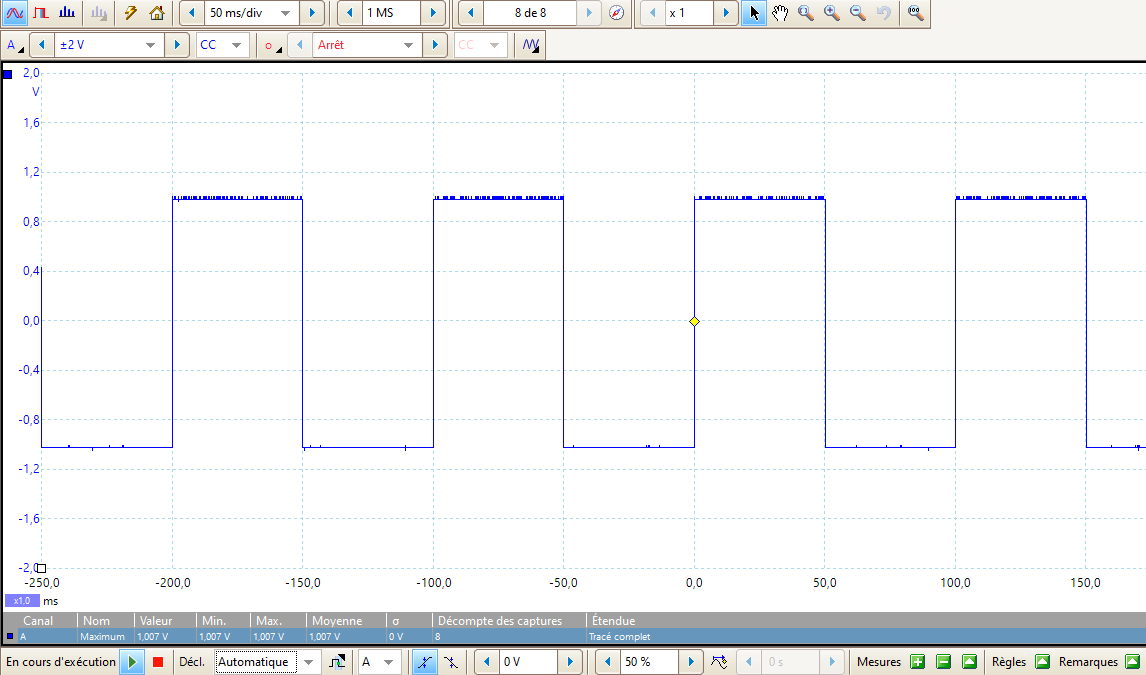
\includegraphics[scale=0.5]{LABO1A/Question_4_2_R.png}
    \caption{Tension aux bornes des 4 résistances}
    \label{fig:my_label}
\end{figure}

\newpage

\subsection{Réflexion analytique et physique}
Considérons le circuit suivant :
\begin{center}
    \begin{circuitikz} \draw
        (0,0) to[sinusoidal voltage source, v=$v_{G}(t)$, i^>=$i(t)$] 
        (0,4) to[resistor, l=$R_G$]
        (4,4) to[generic, l_=$Z_{charge}$, v^<=$v_{charge}(t)$] 
        (4,0) to[resistor, l=$R_e$]
        (2,0) to[resistor, l=$R_e$]
        (0,0) node[ground] {}
        ;
    \end{circuitikz}
\end{center}
Avec:
\begin{itemize}
    \item $v_G(t) = V_m sin(\omega t)$ la source de tension où $V_m = 2V$
    \item la fréquence $f = 50kHz$
    \item $Z_{charge}$ un composant réactif.
\end{itemize}

\Question{
\begin{enumerate}
    \item Quel dipôle devrions nous placer à la place de $Z_charge$ pour que la tension $v_{charge}(t)$ soit en avance de phase sur le courant $i(t)$?\\
    \textcolor{darkblue}{Nous devrions placer une inductance.}
    \item Quel dipôle devrions nous placer à la place de $Z_charge$ pour que la tension $v_{charge}(t)$ soit en retard de phase sur le courant $i(t)$?\\
    \textcolor{darkblue}{Nous devrions placer une capacité.}
    \item Si $Z_{charge}$ est un condensateur, comment doit évoluer la fréquence de la source si l'on veut augmenter le module de la tension $v_{charge}(t)$? Justifiez physiquement ce phénomène.\\
    \textcolor{darkblue}{Le diviseur impédant est en fait un filtre passe-bas. La capacité se comporte comme un circuit ouvert aux BF. Il faut donc que la fréquence soit la plus basse possible.}
    \item Si $Z_{charge}$ est une inductance, comment doit évoluer la fréquence de la source si l'on veut augmenter le module de la tension $v_{charge}(t)$? Justifiez physiquement ce phénomène.\\
    \textcolor{darkblue}{Le diviseur impédant est ici un filtre passe-haut. La capacité se comporte comme un court-circuit aux BF. Il faut donc que la fréquence soit la plus haute possible.}
\end{enumerate}}


\end{document}
%\input{TP1/tp1.tex}
%%% fancy header & foot
\pagestyle{fancy}
\lhead{[ELEC-H-2001] Électricité\\ LABO \no 1B : Circuits réactifs en régime - Phaseurs et impédances \ifthenelse{\boolean{corrige}}{~-- corrigé}{}}
\rhead{v1.0.0\\ page \thepage}
\cfoot{}
%%
\usepackage{placeins}
\pdfinfo{
/Author (Renaud Theunissen et Youssef Agram, ULB -- BEAMS-EE)
/Title (Laboratoire 1B ELEC-H-2001, Circuits réactifs en régime - Phaseurs et impédances)
/ModDate (D:\pdfdate)
}

\hypersetup{
pdftitle={Labo 1A [ELEC-H-2001] Électricité : LABO 1B ELEC-H-2001, Circuits réactifs en régime - Phaseurs et impédances},
pdfauthor={Renaud Theunissen et Youssef Agram, ©2020 ULB - BEAMS-EE},
}


\setlength{\parskip}{0.5cm plus4mm minus3mm} %espacement entre §
\setlength{\parindent}{0pt}


\begin{document}

\tptitle{}{Séance 1B~: Circuits réactifs en régime - Phaseurs et impédances}
\section{But de la manipulation}
Le but de cette séance est de vous familiariser avec le matériel de laboratoire et à développer une approche d'investigation des phénomènes liés aux circuits électrique étudiés dans le cours d'ELEC-H-2001.

Pour ce laboratoire vous aurez besoin des éléments suivants :
\begin{itemize}
    \item Votre PicoScope
    \item Les trois sondes (câbles BNC fournit dans le kit).
    \item Le protoboard
    \item Les résistances $R_e$, $R_i$ et $R_j$
    \item L'inductance $L$
    \item Le condensateur $C_i$
\end{itemize}

\section{Pré-requis}
Pour réaliser cette séance de laboratoire, il vous est recommandé de relire attentivement les sections du syllabus suivantes :
\begin{itemize}
    \item Section 4.3 - Adaptation d'impédance
    \item Sections 5.1 à 5.3 - Loi des mailles et utilisation
    \item Section 7.3 - Phaseurs
    \item Section 7.4 - Impédances et admittances
\end{itemize}

\newpage

\subsection{Mesures de signaux et interprétation - circuit réactif \textbf{RL}}
Réalisez le circuit suivant sur votre \textit{Protoboard}:
\begin{center}
    \begin{circuitikz}\draw
        (0,0) to[sinusoidal voltage source, v=$v_G(t)$, i^>=$i(t)$] (0,4)
        to[resistor, l=$R_G$] (4,4)
        to[inductor, l_=$L$, v^<=$v_{charge}(t)$] (4,0) to[resistor, l=$R_e$] (0,0) node[ground]{};
    \end{circuitikz}
\end{center}
\Question{
En utilisant les outils du logiciel PicoScope 6:\\ 
\begin{enumerate}
    \item Utilisez un canal math pour représenter la tension $V_{charge}(t)$ à partir des signaux de tensions à la sortie du générateur et aux bornes de $R_e$.\\
    \textcolor{darkblue}{Le canal violet représente la tension aux bornes de l'inductance.
    \begin{figure}[h!]
        \centering
        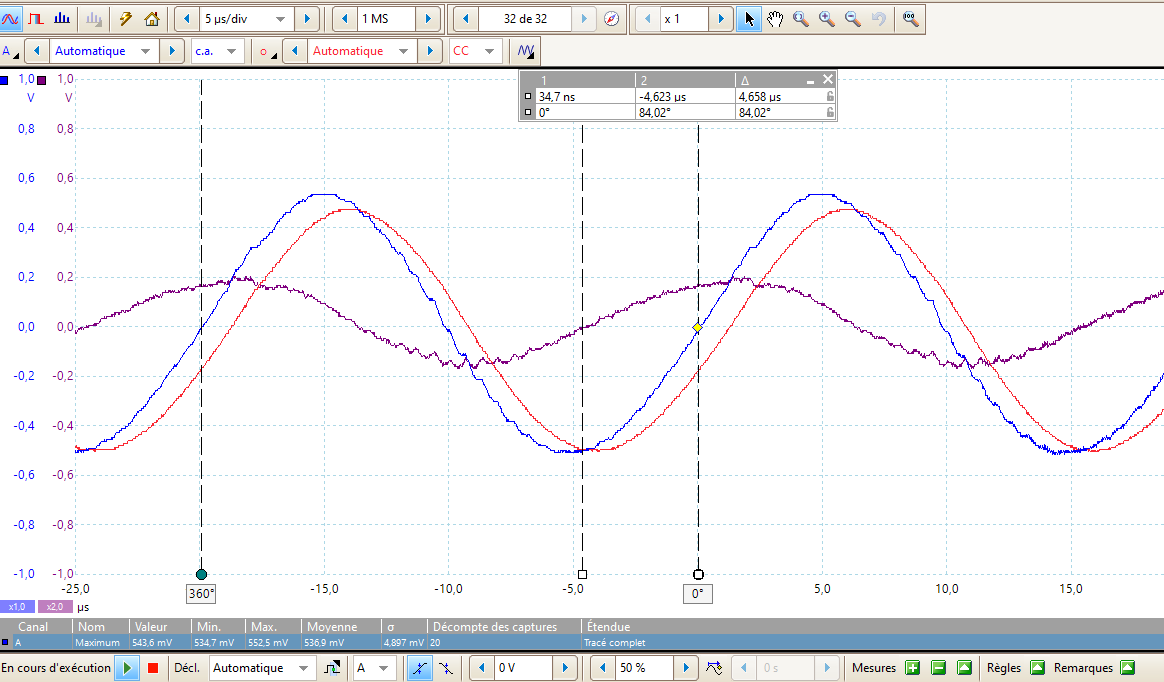
\includegraphics[scale=0.5]{TP2/RL_50k_R.png}
        \caption{Mesure de la tension aux bornes de l'inductance pour $f=50\ kHz$.}
        \label{fig:my_label}
    \end{figure}}
    \item Déterminez la plage de fréquences du signal $v_G(t)$ pour laquelle la tension $v_{charge}(t)$ est maximale.\\
    \textcolor{darkblue}{La transmittance du filtre étant $H(j\omega)=\frac{j\omega L}{R+j\omega L}$, le pole nous donne la fréquence de coupure du filtre: $p=-\frac{R_e}{L}=-909.1 \frac{krad}{s} \longrightarrow f_c=\frac{\omega}{2\pi}=144.7\ kHz$ . On est en présence d'un filtre \textbf{passe-haut}. L'oscilloscope présente un signal coupé aux alentours de 1 kHz et la tension sera maximale pour la plus grande valeur de fréquence i.e. 100 kHz.}
    \item Pour quelle fréquence le déphasage entre $v_G(t)$ et $v_{charge}(t)$ est-il le plus important?\\
    \\
    \FloatBarrier
    \begin{table}[h!]
        \centering
        \textcolor{darkblue}{
        \begin{tabular}{|c|c|c|c|}
        \hline
            & 10 kHz & 50 kHz & 100 kHz  \\
        \hline
        $\Delta \varphi$ & $84.47$°& $84$° & $68.57$°\\
        \hline
        \end{tabular}}
        \caption{Valeurs de déphasage pour différentes fréquences.}
        \label{tab:my_label}
    \end{table}
    \textcolor{darkblue}{Il devient ensuite difficile de mesurer le déphasage pour des fréquences inférieures. Par ailleurs, on devrait retrouver un déphasage de 45° à la fréquence de coupure.}
    \FloatBarrier
    \item Trouvez la valeur de $L$ à partir de la mesure de la tension $v_{charge}(t)$ et de $v_{R_e}(t)$.\\
    \textcolor{darkblue}{On peut trouver la valeur de l'inductance L sur base des amplitudes $V_{charge}$ et $V_{R_e}$ car cette dernière est à l'image du courant qui circule dans la maille:
    $$
     \left\{
                \begin{array}{r c l}
                  \underline{V}_{R_e} & = & R_e\,\underline{I}\\
                  \underline{V}_{charge} & = & j\omega L\,\underline{I}\\
                \end{array}
              \right. \longrightarrow  L=\frac{R_e}{\omega}\frac{V_c}{V_{R_e}}=\frac{200\times0.315}{2\pi\,50\times10^3\times 0.98}\simeq 204.62\ \mu H$$
    Cette méthode est beaucoup plus simple analytiquement qu'utiliser la formule du diviseur impédant.}
\end{enumerate}}
    

\subsection{Mesures de signaux et interprétation - circuit réactif \textbf{RC}}
Réalisez le circuit suivant sur votre \textit{Protoboard}:\\
\begin{center}
    \begin{circuitikz}\draw
        (0,0) to[sinusoidal voltage source, v=$v_G(t)$, i^>=$i(t)$] (0,4)
        to[resistor, l=$R_G$] (4,4)
        to[capacitor, l_=$C_i$, v^<=$v_{charge}(t)$] (4,0) to[resistor, l=$R_e$] (0,0) node[ground]{};
    \end{circuitikz}
\end{center}

En utilisant les outils du logiciel PicoScope 6: 
\Question{
\begin{enumerate}
    \item Utilisez un canal math pour représenter la tension $V_{charge}(t)$ à partir des signaux de tensions à la sortie du générateur et aux bornes de $R_e$.\\
   \begin{figure}[h!]
       \centering
       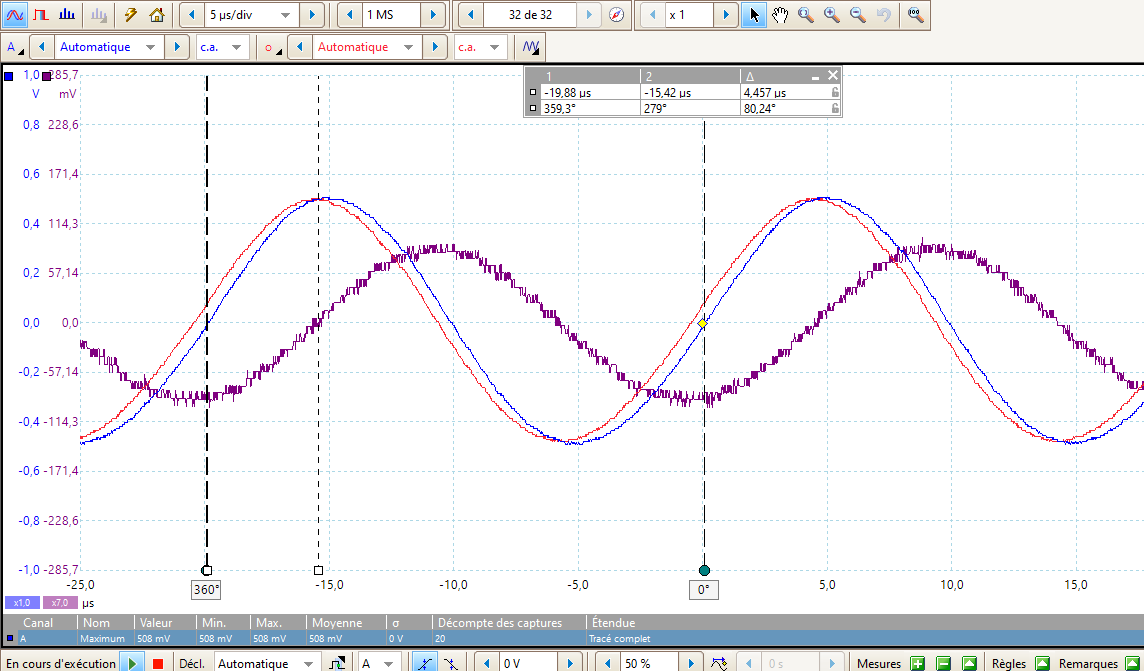
\includegraphics[scale=0.5]{TP2/RC_50k_R.png}
       \caption{Mesure de la tension aux bornes de la capacité pour $f=50\ kHz$.}
       \label{fig:my_label}
   \end{figure}
    \item Déterminez la plage de fréquences du signal $v_G(t)$ pour laquelle la tension $v_{charge}(t)$ est maximale.\\
     \textcolor{darkblue}{La transmittance du filtre étant $H(j\omega)=\frac{1}{1+j\omega RC}$, le pole nous donne la fréquence de coupure du filtre: $p=-\frac{1}{RC} \longrightarrow f_c=7.96\ kHz$ . On est en présence d'un filtre \textbf{passe-bas}. Malgré la fréquence de coupure atteinte, on distingue encore un signal à la fréquence max de la bande passante i.e. 100 kHz. L'amplitude semble être maximale sur la plage $[0\,Hz,100\,Hz]$.}
    \item Pour quelle fréquence le déphasage entre $v_G(t)$ et $v_{charge}(t)$ est-il le plus important?\\
    \FloatBarrier
    \begin{table}[h!]
        \centering
        \textcolor{darkblue}{
        \begin{tabular}{|c|c|c|c|c|c|}
        \hline
            & 100 Hz & 1 kHz & 10 kHz & 50 kHz & 100 kHz  \\
        \hline        $\Delta \varphi$ & $\simeq 0$°& $-8.09$° & $-48.46$° & $-78.95$° & $-85.52$°\\
        \hline
        \end{tabular}}
        \caption{Valeurs de déphasage pour différentes fréquences.}
        \label{tab:my_label}
    \end{table}
    \FloatBarrier
    \textcolor{darkblue}{Le déphasage devrait valoir -45° à la fréquence de coupure.}
    \item Trouvez la valeur de $C_i$ à partir de la mesure de la tension $v_{charge}(t)$ et de $v_{R_e}(t)$.
    \textcolor{darkblue}{On peut trouver la valeur de la capacité similairement:
    $$
     \left\{
                \begin{array}{r c l}
                  \underline{V}_{R_e} & = & R_e\,\underline{I}\\
                  \underline{V}_{charge} & = &\frac{1}{j\omega C}\,\underline{I}\\
                \end{array}
              \right. \longrightarrow  C=\frac{1}{\omega R}\frac{V_{R_e}}{V_{charge}}\simeq0.1 \,\micro F$$
    }
\end{enumerate}}{}

\subsection{Mesures de signaux et interprétation - circuit RLC}
Réalisez le circuit suivant :
\begin{center}
    \begin{circuitikz}\draw
    (0,0) to[sinusoidal voltage source, v=$v_G(t)$, i^>=$i_G(t)$] 
    (0,4)   to[resistor, l=$R_G$] 
    (4,4)   to[inductor, l=$L$] (4,0)
    (4,4)--(6,4)   to[capacitor, l_=$C_i$, v^<=$v_{charge}(t)$]
    (6,0)--(4,0) to[resistor, l=$R_e$] (0,0)   node[ground]{}
    ;
    \end{circuitikz}
\end{center}
Réglez la source de tension avec une amplitude de $V_m=2V$ et une fréquence de $50 kHz$.
\Question{
\begin{enumerate}
    \item Déterminez une plage de fréquence pour laquelle la tension $v_{charge}$ à une amplitude supérieure à la tension $v_{R_e}$.\\
    \textcolor{darkblue}{Nous sommes en présence d'un filtre d'ordre 2. En effet, nous pouvons calculer la fonction de transfert du circuit avec $\underline{V}_{in}$. Il ne faut pas prendre en compte la résistance $R_G$ dans le filtre car les signaux sont mesurés en sortie du générateur. 
    $$
     \left\{
                \begin{array}{r c l}
                  Z_{eq} & = & \frac{Z_L\,Z_C}{Z_L+Z_C}\\
                  \underline{V}_{charge} & = &\frac{Z_{eq}}{Z_{eq}+R_e}\,\underline{V}_{in}\\
                \end{array}
              \right. \longrightarrow H(p)=\frac{pL}{R_e\,(1+p^2LC)+pL}$$ 
              $$H(p)=\frac{pL}{R_eLC\,p^2+Lp+R_e}$$\\
    On a donc 1 zéro à l'origine et 2 pôles complexes conjugués: $p_{1,2}=-\sigma \pm j\omega_d=(-25+j\,211.7)\times 10^3$. La fréquence de résonance vaut donc en principe $\omega_n=\sqrt{\sigma^2+\omega_d^2}=213.171\ kHz$. On a donc un pic de résonance autour de cette fréquence avec une atténuation aux basses et hautes fréquences (filtre passe-bande).\\
    Sur le picoscope, on voit }
              
    \item Que devient l'amplitude de $v_{charge}$ pour une fréquence $f=500Hz$? Justifiez physiquement ce résultat.
    \item Donnez une plage de fréquence pour laquelle le déphasage entre $v_{charge}$ et $v_{R_e}$ est maximal.
\end{enumerate}}{}

\end{document}
%%% fancy header & foot
\pagestyle{fancy}
\lhead{[ELEC-H-2001] Électricité\\ LABO \no 2 : Séance 2~: Les circuits réactifs en transitoire \ifthenelse{\boolean{corrige}}{~-- corrigé}{}}
\rhead{v1.0.0\\ page \thepage}
\cfoot{}
%%
\usepackage{placeins}
\pdfinfo{
/Author (Renaud Theunissen & Youssef Agram, ULB -- BEAMS-EE)
/Title (Laboratoire 2 ELEC-H-2001, Séance 2~: Les circuits réactifs en transitoire)
/ModDate (D:\pdfdate)
}

\hypersetup{
pdftitle={Labo 2 [ELEC-H-2001] Électricité : LABO 2~: Les circuits réactifs en transitoire},
pdfauthor={Renaud Theunissen & Youssef Agram, ©2020 ULB - BEAMS-EE},
}


\setlength{\parskip}{0.5cm plus4mm minus3mm} %espacement entre §
\setlength{\parindent}{0pt}



\begin{document}

\tptitle{}{Séance 2~: Les circuits réactifs en transitoire}
Le but de cette séance est de vous amener à expliquer et comprendre les phénomènes transitoires de circuits réactifs (à l'aide d'une onde carré à basse fréquence).
Mesurer les comportements des dipôles réactifs soumis à certaines sollicitations. 
Cette séance nous permet également de tenir compte des imperfections des dipôles que nous utilisons par rapport au cas idéal que nous traitons dans les exercices.

\section{Pré-requis}
Avant la séance, vous aurez lu attentivement l'énoncé de la manipulation. Vous aurez par ailleurs relu les chapitres et sections suivants:

\begin{itemize}
	\item Chapitre 2 - Dipôles idéaux
	\begin{itemize}
	    \item Section 2.2 - Dipôles réels >< Dipôles idéaux
	    \item Section 2.3 - Charges idéales : trois effets physiques
	    \item Section 2.6 - Sources idéales
	\end{itemize}
	\item Chapitre 5 - Résoudre un circuit réactif dans le domaine temporel
	\item Chapitre 6 - Résoudre un circuit réactif dans le domaine temporel
	\begin{itemize}
	    \item Section 6.1 - Éléments réactifs : Rappels 
		\item Section 6.2 - Analyse temporelle du circuit RC (source en échelons)
		\item Section 6.3 - Analyse temporelle du circuit RL (source en échelons)
		\item Section 6.5 - Analyse temporelle du circuit RL (source sinusoïdale avec échelon)
		\item Section 6.6 - Analyse temporelle du circuit RLC
	\end{itemize}

\end{itemize}

\vspace{5pt}

\newpage
\section{Préliminaire théorique}
Soit le circuit ci-dessous alimenté par une source de tension continue $V_S$ qui délivre un courant $I$. En tenant compte de l'existence d'un interrupteur représenté par $T_0$ qui sera fermé au temps $t_0 = 0s$, de $R$ une résistance et $L$ une inductance tous deux de valeurs quelconques :
\begin{center}
\begin{circuitikz} \draw
    (0,0)	to[battery1, v=$V_S$, invert, i^>=$I$]		
    (0,4)	to[closing switch, l=$T_0$]		
    (2,4)	to[R, l=$R$]					
    (4,4)	to[L, l=$L$, v_<=$v_L$]					(4,0)--(0,0) node[ground]{}
;
\end{circuitikz}
\end{center}
\Question{
\newline
\begin{enumerate}
    \item Déterminez l'expression analytique de $v_L(t)$ pour tous temps $t\in [T_{-\infty}; T_1]$ avec $T_1 >> T_0$.
    \item Déterminez la constante de temps $\tau$ pour ce circuit?
    \item Comment affecterai l'ajout d'inductances en séries sur la constante de temps $\tau$?
\end{enumerate}
}
{%C
}

\newpage
\section{Partie pratique}
\subsection{Réflexion analytique et physique}
Nous désirons observer des phénomènes transitoires. 
\Question{
\newline
\begin{enumerate}
    \item Quels types de dipôles sont strictement nécessaire pour observer de tels phénomènes? Justifiez à l'aide de la loi du/des dipôle(s) cette affirmation.
    \item Sans interrupteur, comment pourrions-nous observer un effet similaire au régime transitoire pour le circuit suivant :
    \begin{center}
    \begin{circuitikz} \draw
        (0,0)	to[battery1, v=$V_S$, invert, i^>=$I$]		
        (0,4)	to[closing switch, l=$T_0$]		
        (2,4)	to[R, l=$R$]					
        (4,4)	to[L, l=$L$, v_<=$v_L$]				(4,0)--(0,0) node[ground]{}
        ;
    \end{circuitikz}
    \end{center}
\end{enumerate}
}
{%C
}
\newpage
\subsection{Réflexion analytique et physique - Circuit RL}
Considérons le circuit suivant :
\begin{center}
\begin{circuitikz} \draw
        (0,0)	to[square voltage source, v=$v_G(t)$, i^>=$i(t)$]		
        (0,4)	to[R, l=$R_G$]
        (4,4)	to[L, l=$L$]	
        (4,0)   to[R, l=$R_e$] 
        (0,0)   node[ground]{}
        ;
\end{circuitikz}
\end{center}
\Question{
\newline
\begin{enumerate}
    \item Après combien de temps le courant dans le circuit aura atteint 95\% de sa valeur maximale?
    \item Comment régleriez-vous $v_G(t)$ pour que le régime permanent ne s'établisse jamais dans ce circuit? 
\end{enumerate}
}
{%C
}
\newpage
\subsection{Mesures de signaux et interprétation - circuit RL}
Réalisez le circuit suivant sur votre ProtoBoard :
\begin{center}
\begin{circuitikz} \draw
        (0,0)	to[voltage source, v=$v_G(t)$, i^>=$i(t)$]		
        (0,4)	to[R, l=$R_G$]					
        (4,4)	to[L, l=$L$, v_<=$v_L$]	
        (4,0)   to[R, l=$R_e$] 
        (0,0)   node[ground]{}
        ;
\end{circuitikz}
\end{center}
Avec :
\begin{itemize}
    \item $v_G(t)$ une source de tension 
    \item $R_G = 600\Omega$ la résistance de sortie du générateur du PicoScope
    \item $L = 220$µH l'inductance de votre kit de laboratoire
    \item $R_e = 200\Omega$ la résistance étalon
\end{itemize}
\Question{
\newline
\begin{enumerate}
    \item Paramétrez la source de tension de votre générateur pour obtenir une situation similaire à une source de tension continue suivie d'un interrupteur.
    \item Mesurez le temps nécessaire à l'atténuation du régime transitoire de ce circuit.
    \item Comparez cette valeur avec le constante de temps du circuit. Quelle conclusion pouvez-vous en tirer?
    \item Pour une source de fréquence deux fois moins importante, pensez-vous que constante de temps aura une valeur plus basse? Justifiez analytiquement.
\end{enumerate}

}
{%C
}
\newpage
\subsection{Réflexion analytique et physique - Circuit RC}
Considérons le circuit suivant :
\begin{center}
\begin{circuitikz} \draw
        (0,0)	to[square voltage source, v=$v_G(t)$, i^>=$i(t)$]		
        (0,4)	to[R, l=$R_G$]
        (4,4)	to[C, l=$C_i$]	
        (4,0)   to[R, l=$R_e$] 
        (0,0)   node[ground]{}
        ;
\end{circuitikz}
\end{center}
\Question{
\newline
\begin{enumerate}
    \item Après combien de temps le courant dans le circuit aura atteint 63\% de sa valeur maximale?
    \item Comment régleriez-vous $v_G(t)$ pour que le régime permanent ne s'établisse jamais dans ce circuit? 
\end{enumerate}
}
{%C
}
\newpage
\subsection{Mesures de signaux et interprétation - circuit RC}
Réalisez le circuit suivant sur votre ProtoBoard :
\begin{center}
\begin{circuitikz} \draw
        (0,0)	to[voltage source, v=$v_G(t)$, i^>=$i(t)$]		
        (0,4)	to[R, l=$R_G$]					
        (4,4)	to[C, l=$C_i$, v_<=$v_C$]	
        (4,0)   to[R, l=$R_e$] 
        (0,0)   node[ground]{}
        ;
\end{circuitikz}
\end{center}
Avec :
\begin{itemize}
    \item $v_G(t)$ une source de tension 
    \item $R_G = 600\Omega$ la résistance de sortie du générateur du PicoScope
    \item $C_i = 0,1$ µF le condensateur de votre kit de laboratoire
    \item $R_e = 200\Omega$ la résistance étalon
\end{itemize}
\Question{
\newline
\begin{enumerate}
    \item Paramétrez la source de tension de votre générateur pour obtenir une situation similaire à une source de tension continue suivie d'un interrupteur.
    \item Mesurez le temps nécessaire à l'atténuation du régime transitoire de ce circuit.
    \item Comparez cette valeur avec le constante de temps du circuit. Quelle conclusion pouvez-vous en tirer?
    \item Si la source de tension $v_G(t)$ a une amplitude deux fois plus importante, pensez-vous que cela augmentera la valeur de la constante de temps? Justifiez analytiquement.
\end{enumerate}
}
{%C
}

\end{document}
%%% fancy header & foot
\pagestyle{fancy}
\lhead{[ELEC-H-2001] Électricité\\ LABO \no 3 : Théorème de Thévenin et adaptation d'impédance \ifthenelse{\boolean{corrige}}{~-- corrigé}{}}
\rhead{v1.0.0\\ page \thepage}
\cfoot{}
%%

\pdfinfo{
/Author (Renaud Theunissen et Youssef Agram, ULB -- BEAMS-EE)
/Title (Laboratoire 3 ELEC-H-2001, Théorème de Thévenin et adaptation d'impédance)
/ModDate (D:\pdfdate)
}

\hypersetup{
pdftitle={Labo 3 [ELEC-H-2001] Électricité : LABO 3 ELEC-H-2001, Théorème de Thévenin et adaptation d'impédance},
pdfauthor={Renaud Theunissen et Youssef Agram, ©2020 ULB - BEAMS-EE},}

\setlength{\parskip}{0.5cm plus4mm minus3mm} %espacement entre §
\setlength{\parindent}{0pt}


\begin{document}
\long\def\nothx/*#1*/{}
\tptitle{}{Séance 3~: Théorème de Thévenin et adaptation d'impédance}
\section{But de la manipulation}
L'objectif de cette dernière séance de laboratoire est de vous permettre d'aborder les équivalents de Thévenin et d'en tester l'efficacité ainsi que les limites.
Vous serez également amené à utiliser à nouveau les critères d'adaptation d'impédance pour considérer les charges que nous pourrons ou non brancher aux circuits proposés.

\section{Pré-requis}
Avant la séance, vous aurez lu attentivement l'énoncé de la manipulation. Vous aurez par ailleurs relu les chapitres et sections suivants:
\begin{itemize}
	\item Chapitre 4 - Équivalence de Thévenin et adaptation d'impédance
		\begin{itemize}
		\item Section 4.1 - Circuit équivalents et théorèmes de Thévenin et Norton
		\item Section 4.2 - Impédance d'entrée, impédance de sortie (et fem à vide)
		\item Section 4.3 - Adaptation d'impédance
		\end{itemize}
	\item Chapitre 5 - Résoudre un circuit : procédure de base et accélérateurs
		\begin{itemize}
		\item Section 5.1.2 - Connexions série et parallèle
			\begin{itemize}
			\item Section 5.4 Illustration : Diviseur résistif (étendu aux impédances) 
			\item Section 5.5 Équivalences série et parallèle
			\item Section 5.6 Utilisation des théorèmes de Thévenin et Norton pour résoudre un circuit
			\end{itemize}
		\end{itemize}
	\item Chapitre 7 - Résoudre un circuit réactif dans le domaine fréquentiel
		\begin{itemize}
		\item Section 7.3 - Phaseurs
		\item Section 7.4 - Impédances et admittances
		\end{itemize}
\end{itemize}

\vspace{5pt}

\newpage

\section{Préliminaire Théorique}
\subsection{Équivalent de Thévenin et théorème de superposition}

Soit le circuit suivant :

\begin{center}
\begin{circuitikz} \draw
    (0,0)	to[battery1, v=$V_1$, invert, i^>=$I$]		
    (0,5)	to[R, l=$R$]		
    (2,5)	-- (2,4)--
    (1,4)   to[R, l=$R$]
    (1,2)--(3,2)
            to[R, l_=$R$] (3,4)--(2,4)--(2,5)--
    (5,5)   to[battery1, v=$V_2$, invert] 
    (5,3)   to[R, l_=$R$] 
    (5,1)--(4,1)
        to[R, l=$R$] (2,1)--(2,0)
        to[R, l_=$R$] (4,0)--(4,1)
    (2,1)   to[R, l^=$R$] (0,1)--
    (0,0) node[ground]{}
    (2,2)--(2,1)
    (2,4) to[open, v^<=$V_3$] (2,2)
;
\end{circuitikz}
\end{center}
\Question{
\newline
\begin{itemize}
    \item Déterminez l'équivalent de Thévenin ($V_{Th}$ et $R_{Th}$) de ce circuit vu par la source $V_1$ en fonction de $R$, $V_2$ et $I$.
    \item Déterminez la tension $V_3$ à l'aide du théorème de superposition.
\end{itemize}
}
{%C
}
\newpage
\section{Partie pratique}
\subsection{Réflexion analytique et physique - Circuit résistif}
Considérons le circuit suivant :
\begin{center}
\begin{circuitikz} \draw
(0,0)   to[sinusoidal voltage source, v>=$v_G(t)$, invert, i^>=$i(t)$] 	(0,6)
		to[R, l=$R_G$] (2,6)
		to[R, l=$R$] (4,6)
		(2,6)--(2,7)
		to[R, l=$R$] (4,7)--(4,5)
		to[R, l_=$R$] (2,5)--(2,6)
		(4,6)--(5,6)--(5,7)
		to[R, l=$R$] (7,7)--(7,5)
		to[R, l_=$R$] (5,5)--(5,6)
		(7,6)--(8,6)
		to[generic, l=$R_{charge}$](8,0)--(0,0)
		node[ground]{}	
		node[ocirc] (A) at (8,6) {A}
        node[ocirc] (B) at (8,0) {B}
;
\end{circuitikz}
\end{center}
\Question
{%Question
\newline
\begin{enumerate}
    \item Déterminez l'équivalent de Thévenin vu depuis $R_{charge}$ (entre les point A et B).
    \item Pensez-vous que le type de source peut influencer l'équivalent de Thévenin de ce circuit?
    \item Quelle devra être la valeur de $R_{charge}$ pour que la tension à ces bornes soit égale à 25\% de celle de $v_G$?
\end{enumerate}
}
{%C
}

\newpage
\subsection{Mesures de signaux et interprétation - Circuit résistif}

Soit le circuit suivant avec :

\begin{itemize}
    \item $R_x$ qui est la mise en série de la résistance $R_{x_1}$ et $R_{x_2}$.
    \item $R_i$ et $R_e$ qui ont été déterminées dans les séances précédentes.
    \item La source de tension $v_G(t)$ est une source de 2V d'amplitude et de forme sinusoïde (la pulsation importe peu).
\end{itemize}
\begin{center}
\begin{circuitikz} \draw
(0,0)   to[sinusoidal voltage source, v>=$v_G(t)$, invert, i^>=$i(t)$] 	(0,6)
		to[R, l=$R_G$] (2,6)
		to[R, l=$R_i$] (4,6)
		(2,6)--(2,7)
		to[R, l=$R_x$] (4,7)--(4,5)
		to[R, l_=$R_e$] (2,5)--(2,6)
		(4,6)--(5,6)--(5,7)
		to[R, l=$R_i$] (7,7)--(7,5)
		to[R, l_=$R_i$] (5,5)--(5,6)
		(7,6)--(8,6)
		to[generic, l=$R_{charge}$](8,0)--(0,0)
		node[ground]{}	
		node[ocirc] (A) at (8,6) {A}
        node[ocirc] (B) at (8,0) {B}
;
\end{circuitikz}
\end{center}

\Question {
\newline
\begin{enumerate}
    \item Proposez une procédure pour déterminer la résistance $R_x$ et donnez sa valeur.
    \item En utilisant les valeurs des résistances $R_i$ et $R_e$ trouvées précédemment ainsi que celle de $R_x$, déterminez l'équivalent de Thévenin du circuit proposé.
    \item Quelle sera la tension appliquée sur $R_{charge}$ si cette dernière est égale à $200\Omega$ (donc $R_{charge}$=$R_e$)?
    \item Proposez et tester un montage équivalent à ce dernier mais en utilisant qu'une seule résistance en plus de $R_G$.
\end{enumerate}
}
{%C
}
\newpage
\subsection{Réflexion analytique et physique - Circuit réactif}
Soit le circuit suivant avec:
\begin{itemize}
    \item $R_G = 600\Omega$ la résistance de sortie du générateur.
    \item $C_i = 0,1$µF, $C_j = 22$nF et $C_k = 4,7$nF.
    \item La source de tension $v_G(t)$ est une source de 2V d'amplitude et de forme sinusoïde (la pulsation importe peu).
\end{itemize}
\begin{center}
\begin{circuitikz} \draw
(0,0)   to[sV, v>=$v_G(t)$] 	(0,4)
		to[R, l_=$R_G$] (2,4)--(3,4)--(3,5)
		to[C, l_=$C_i$] (5,5)--(5,4)
(3,4)--(3,3)
        to[C, l_=$C_k$] (5,3)--(5,4)
        to[C, l_=$C_j$] (7,4)--(8,4)
        to[generic, l=$R_{Charge}$] (8,0)--(0,0)
        node[ground]{}
        node[ocirc] (A) at (8,4) {A}
        node[ocirc] (B) at (8,0) {B}
;
\end{circuitikz}
\end{center}
\Question
{%Question
\newline
\begin{enumerate}
    \item Déterminez l'équivalent de Thévenin vu depuis $R_{Charge}$ (entre les point A et B).
    \item Si $R_{Charge}$ est égale à $R_e$, calculez sa différence de potentiel $V_{R_e}$ à partir de votre équivalent de Thévenin.
    \item Si nous plaçons une inductance à la place de la charge, pour quelles fréquences (hautes ou basses) aurons nous une $v_{Charge}$ maximale? Justifiez physiquement.
\end{enumerate}
}
{%C
}

%Pour l'année prochaine celle-ci!
\newpage
\subsection{Mesures de signaux et interprétation - Circuit réactif}
Soit le circuit suivant avec :
\begin{itemize}
    \item $R_G = 600\Omega$ la résistance de sortie du générateur.
    \item $C_i = 0,1$µF, $C_j = 22$nF et $C_k = 4,7$nF.
    \item La source de tension $v_G(t)$ est une source de 2V d'amplitude et de forme sinusoïde à une fréquence de $100$ kHz.
\end{itemize}
\begin{center}
\begin{circuitikz} \draw
(0,0)   to[sV, v>=$v_G(t)$] 	(0,4)
		to[R, l_=$R_G$] (2,4)--(3,4)--(3,5)
		to[C, l_=$C_i$] (5,5)--(5,4)
(3,4)--(3,3)
        to[C, l_=$C_k$] (5,3)--(5,4)
        to[C, l_=$C_j$] (7,4)--(8,4)
        to[generic, l=$R_e$] (8,0)--(0,0)
        node[ground]{}
;
\end{circuitikz}
\end{center}


\Question
{%Question
\newline
\begin{enumerate}
    \item Vérifiez qu'avec l'équivalent de Thévenin que vous avez déterminé précédemment, vous mesurez une différence de potentiel $V_{R_e}$ attendue.
    \item Obtiendriez-vous la même valeur si les condensateurs $C_i$ et $C_j$ étaient permutés comme proposé ci-dessous?
    \begin{center}
\begin{circuitikz} \draw
(0,0)   to[sV, v>=$v_G(t)$] 	(0,4)
		to[R, l_=$R_G$] (2,4)--(3,4)--(3,5)
		to[C, l_=$C_j$] (5,5)--(5,4)
(3,4)--(3,3)
        to[C, l_=$C_k$] (5,3)--(5,4)
        to[C, l_=$C_i$] (7,4)--(8,4)
        to[generic, l=$R_e$] (8,0)--(0,0)
        node[ground]{}
;
\end{circuitikz}
\end{center}
    \item En utilisant une fréquence de $50$kHz pour la source, quelle valeur obtenez-vous pour $V_{R_e}$? Justifiez en discutant la validité de l'équivalent de Thévenin entre ce cas et le précédent.
    \item Pour quelle fréquence obtiendriez-vous la même valeur pour $V_{R_e}$ que dans le cas précédent? 
\end{enumerate}
}
{%C
}

\end{document}
%%% fancy header & foot
\pagestyle{fancy}
\lhead{[ELEC-H-2001] Électricité  \ifthenelse{\boolean{corrige}}{~-- corrigé}{}}
\rhead{v1.0.2\\ page \thepage}
\cfoot{}
%%

\pdfinfo{
/Author (Raoul Sommeillier, ULB -- BEAMS)
/Title (ELEC-H-2001, Théorie des champs Électrostatique : champ et potentiel dans le vide)
/ModDate (D:\pdfdate)
}

\hypersetup{
pdftitle={[ELEC-H-2001] Électricité Théorie des champs\\Électrostatique : champ et potentiel dans le vide},
pdfauthor={Raoul Sommeillier, ©2018 ULB - BEAMS  },
%pdfsubject={Théorie des champs\\Électrostatique : champ et potentiel dans le vide}
}

%\date{\vspace{-1cm}\mydate\today}
%\title{\vspace{-2cm} Labo \no 6\\ Électronique appliquée [ELEC-H-301]\\Réalisation d'un ampli à transistor\ifthenelse{\boolean{corrige}}{~\\Corrigé}{}}

%\author{\vspace{-1cm}}%\textsc{Yannick Allard}}

\setlength{\parskip}{0.5cm plus4mm minus3mm} %espacement entre §
\setlength{\parindent}{0pt}


\begin{document}

\tptitle{}{Électrostatique : champ et potentiel dans le vide}

\section{Pré-requis et objectif de la séance}
Avant cette séance, il est préférable d'avoir lu attentivement cet énoncé et revu les chapitres du cours couvrant la théorie vue dans les 4 premières séances d'exercices en Théorie des Circuits.

Les compétences devant être développées par l'étudiant à la fin de cette séance sont en particulier:
\begin{itemize}
	\item Analyser un circuit quelconque et combiner vos connaissances afin de sélectionner la procédure adéquate pour le résoudre
	\item Driller vos connaissances et savoir-faire sur les matières vues précédemment aux séances d'exercices 1 à 4, à savoir: les impédances, les circuits passifs ou réactifs à une ou plusieurs source(s) continue(s) ou alternative(s) en régime transitoire ou établi, les lois de Kirchhoff, les théorèmes de Thévenin et de superposition, l'adaptation d'impédance, le formalisme des phaseurs, etc.  
\end{itemize}

Cet énoncé étant long, vous aurez l'occasion de travailler dessus avec vos assistants à la fin des séances de laboratoire.
\vspace{5pt}

\newpage

\section{Exercices}
\subsection{Soient quatre charges $q_{1}$, $q_{2}$, $q_{3}$, $q_{4}$, disposées de manière à former un carré de côté de longueur $a$.}
\begin{figure}[h!]
    \centering
    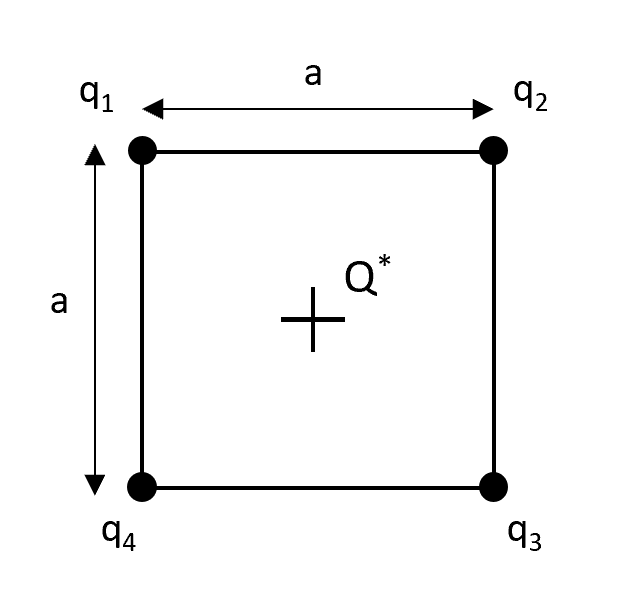
\includegraphics[width = 8cm]{TP5/Tp5_Q1.PNG}
    \caption{Répartition des quatre charges}
    \label{fig:Q1Enonce}
\end{figure}
\Question{ Si les charges ont une même valeur (par exemple: $q_1 = q_2 = q_3 = q_4 = +q$), calculez :
    \begin{itemize}
        \item Le potentiel électrique $\mathbf{V}$ généré par ces dernières au centre du carré.
        \item La force résultante $\mathcal{F}_{res}$ qu'exercent ces quatre charges sur une charge témoin $\mathbf{Q^*}$ placée au centre du carré.
        \item Le travail $\mathcal{W}$ nécessaire pour amener la charge témoin $\mathbf{Q^*}$ d'un point infiniment éloigné jusqu'au centre du carré.
        \item Que devient cette force si une des charges positionnées aux sommets du carré venait à être retirée?
    \end{itemize}
    }
    {}

\Question{Si les charges sont alternées en signe (par exemple : $q_1 = q_3 = +q$ et $q_2 = q_4 = -q$), calculez : 
    \begin{itemize}
        \item Le potentiel électrique $\mathbf{V}$ généré par ces dernières au centre du carré.
        \item La force résultante $\mathcal{F}_{res}$ qu'exercent ces quatre charges sur une charge témoin $\mathbf{Q^*}$ placée au centre du carré.
        \item Le travail $\mathcal{W}$ nécessaire pour amener la charge témoin $\mathbf{Q^*}$ d'un point infiniment éloigné jusqu'au centre du carré.
        \item Que devient cette force si une des charges positionnées aux sommets du carré venait à être retirée?
    \end{itemize}
    }
    {}

\subsection{On considère deux charges Q et -Q distantes d'une longueur s. Les charges sont alignées suivant l'axe x et symétriquement par rapport à l'origine du système d'axes, tel que représenté sur le schéma ci-dessous:}
\begin{figure}[h!]
    \centering
    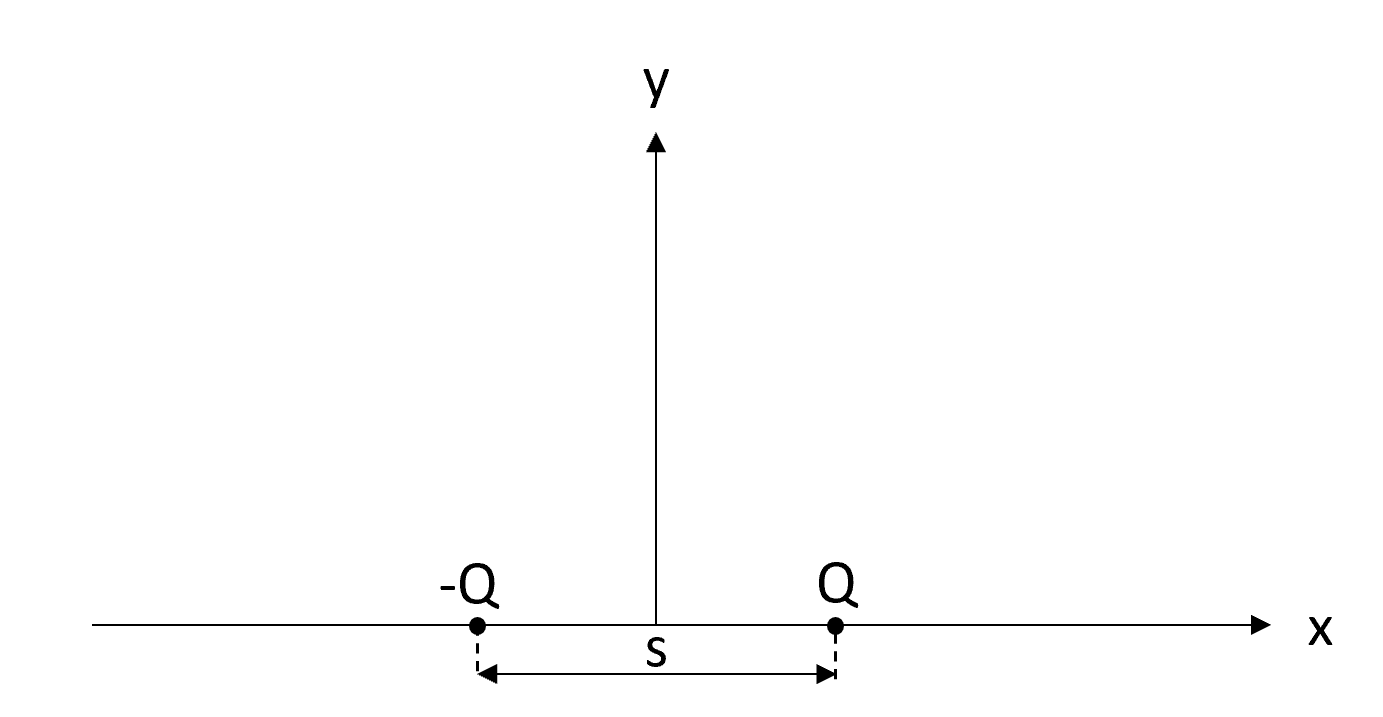
\includegraphics[width = 8cm]{TP5/Tp5_Q2.PNG}
    \caption{Disposition des charges}
    \label{fig:Q2Ennonce}
\end{figure}
\Question{
\begin{itemize}
    \item Déterminez l'expression analytique du champ électrique $\mathbf{E}$ selon l'axe $x$ puis selon l'axe $y$
    \item Simplifiez ces expressions en considérant que la distance aux charges est beaucoup plus grande que $s$ (approximation dipolaire).
    \item Dessinez l'allure des lignes de champ dans le plan xy.
\end{itemize} 
}
{}

\subsection{Considérons une sphère de rayon a portant une charge \textit{totale} Q.}
\Question{Déterminez analytiquement la répartition du potentiel électrique $\mathbf{V}$ et du champ électrique associé $\Vec{E}$ pour tous rayon partant du centre de la sphère jusqu'à l'infini pour les distributions de charge suivantes:
\begin{itemize}
    \item Si la charge $\mathbf{Q}$ est répartie uniformément en volume dans la sphère.
    \item Si la charge $\mathbf{Q}$ est répartie uniformément en surface de la sphère.
    \item Si la charge $\mathbf{Q}$ est répartie dans le volume de la sphère suivant une loi proportionnelle à $R^2$.
\end{itemize}
}
{}
\subsection{Soit un anneau circulaire \textit{filiforme} de diamètre \textit{d} portant une densité de charge linéaire et uniforme $\rho_L$ en $C/m$.}
\Question{Déterminez le potentiel électrique $\mathbf{V}$ et le champ électrique $\Vec{E}$ au centre de cet anneau.}
{}


%QUESTION 9
\Question{
\textit{Résoudre ce circuit où $E_S=10V$. On ferme le premier interrupteur au temps $t=T_1$, puis le second au temps $t=T_2$.\\
On supposera le temps $T_2-T_1$ bien plus grands que les constantes de temps de ce circuit.}
\begin{center}
\begin{circuitikz} \draw
(0,0)   node [ground] {}
		to [american voltage source, v=$E$, invert] 		(0,3)
		to [closing switch, l=$T_1$]				(2,3)
		to [R, l=$R$]								(5,3)
		to [C, l=$C$]								(5,0)
		--(0,0)
(5,3)	to[closing switch, l=$T_2$]					(7,3)
		to [R, l=$R_2$]								(7,0)--(5,0)
;
\end{circuitikz}
\end{center}
}
{
Avant $T_2$, c'est le même circuit que la question 3 de cet exercice: $v_C(t)=E_S(1-e^{\frac{-t}{RC}})$.\\
Après $T_2$, c'est le même exercice que le 2.6 du TP2.
}

%QUESTION 2.2.
\subsection{Question de l'Examen de Janvier 2013}
Soit le circuit suivant
\begin{center}
\begin{circuitikz} \draw
(0,0)   node [ground] {}
		to	 [american voltage source, v=$E$, invert]	(0,2)
		to	 [R, l=$r$]							(0,4)--(2,4)
(2,0)	to	 [american voltage source, v=$2E$, invert]	(2,2)
		to	 [R, l=$r$]							(2,4)--(4,4)
(4,0)	to	 [american voltage source, v=$3E$, invert]	(4,2)
		to	 [R, l=$r$]							(4,4)--(6,4)
(6,0)		to	 [american voltage source, v=$4E$, invert]	(6,2)
		to	 [R, l=$r$]							(6,4)
		to	 [closing switch]					(8,4)
		to   [R, l=$R$]							(8,2)
		to   [C, l=$C$]							(8,0)--(0,0)	
;
\end{circuitikz}
\end{center}

Où $E=20V$, $r=4\Omega$, $R=1\Omega$ et $0,1F$.\\
Avant $t=0$, l'interrupteur est ouvert. On ferme l'interrupteur à l'instant $t=0$. La charge initiale de la capacité est nulle.\\

Après une prise de mesure, on a relevé les deux courbes suivantes où l'axe des abscisses est le temps $[s]$ (une graduation vaut $0,2s$) et l'axe des ordonnées est le courant $[A]$ ou la tension $[V]$.
\begin{center}
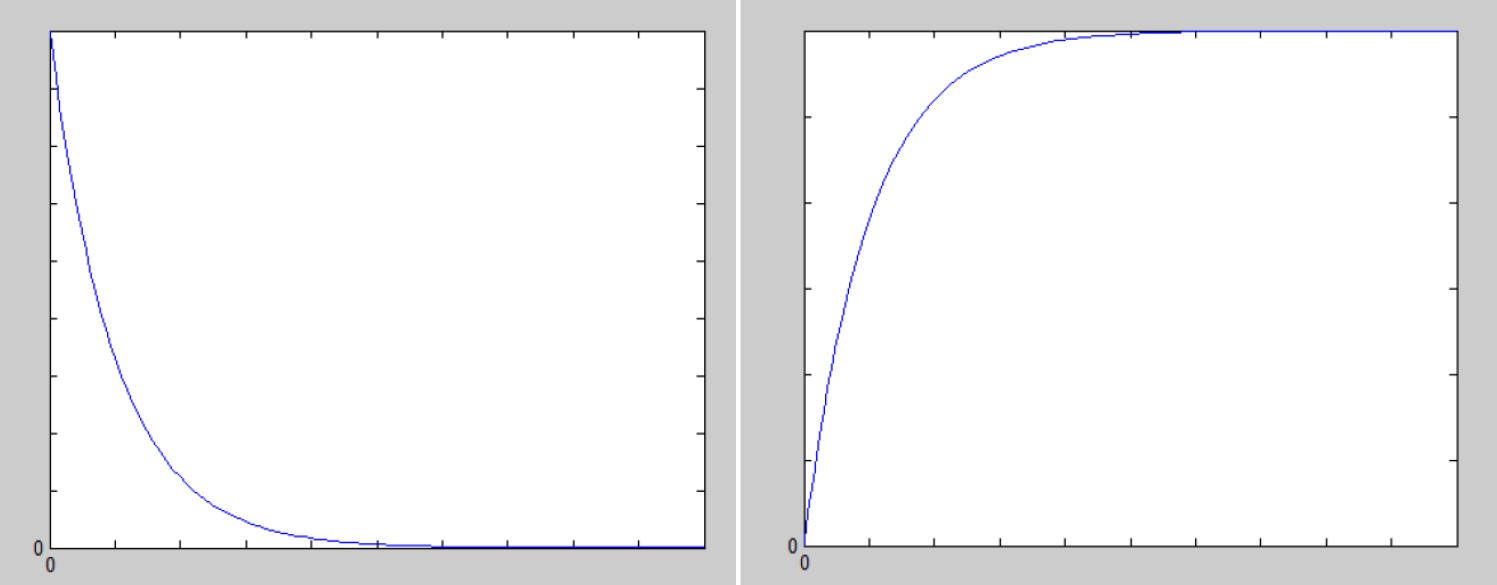
\includegraphics[scale=0.4]{TP5/RC.PNG}
\end{center}

%QUESTION 1.1.
\Question
{
%question
\textit{Identifiez l'élément du schéma (source(s), capacité, resistance(s)) auquel se rapportent ces deux graphes.\\
Identifiez la grandeur (tension(s) ou courant(s)) présente sur l'ordonnée pour chaque courbe.}
}
{
\textbf{Elément:} La capacité\\

\textbf{A droite:}\\
Il s'agit de la tension aux bornes du condensateur $v_C(t)$.\\

Vérification numérique après résolution de la Question 1.4.:\\
$v_C(t)=\frac{5E}{2}(1-\exp{(-\frac{t}{C(R+r/4)})})=50(1-\exp{(-\frac{t}{0,2})}) [V]$ avec une tension initiale $v_C(0-)=v_C(0+)=0V$ et une tension de régime $v_C(\infty)=50V$\\


\textbf{A gauche:}\\
Il s'agit de l'intensité de courant $i(t)$ traversant le condensateur.\\

Vérification numérique après résolution de la Question 1.4.:\\
$i(t)=\frac{10E}{4R+r}exp{(-\frac{t}{C(R+r/4)})}=25 exp{(-\frac{t}{0,2})} [A]$ avec $i(0-)=0A$, $i(0+)=25A$ et $i(\infty)=0A$.
}


%QUESTION 1.2.
\Question
{
%question
\textit{Sur base de ce graphique, déterminer la valeur de la constante de temps $\tau$ du circuit.}
}
{
La constante de temps $\tau$ est par définition le temps nécessaire à la tension aux bornes du condensateur pour atteindre $63\%$ de sa valeur de régime:
$$v_C(\tau)=v_C(\infty)(1-\exp{(-1}))\cong 0,63v_C(\infty)$$

Graphiquement, il suffit de tracer une ligne horizontale passant par $0,63\times 50=31,5V$.\\ L'intersection avec le graphique de $v_C(t)$ donne $\tau=0,2s$.\\

Il était également possible d'utiliser la méthode graphique de la tangente à l'origine (moins précis).

Vérification numérique après résolution:
$$\tau=C(R+\frac{r}{4})=0,1.(1+\frac{4}{4})=0,2s$$
}

%QUESTION 1.3.
\Question
{
%question
\textit{Déterminez les paramètres $R_{th}$ et $V_{th}$ de l'équivalent de Thévenin du circuit vu aux bornes du condensateur.}
}
{
\fbox{$R_{th}$}\\
Pour trouver la résistance équivalente de Thévenin, il faut court-circuiter les sources du circuit. (1 point)

\begin{center}
\begin{circuitikz}[scale=0.6] \draw
(0,0)   node [ground] {}
		to	 [short]	(0,2)
		to	 [R, l=$r$]							(0,4)--(2,4)
(2,0)	to	 [short]	(2,2)
		to	 [R, l=$r$]							(2,4)--(4,4)
(4,0)	to	 [short]	(4,2)
		to	 [R, l=$r$]							(4,4)--(6,4)
(6,0)	to	 [short]	(6,2)
		to	 [R, l=$r$]							(6,4)
		to	 [short]					(8,4)
		to   [R, l=$R$]							(8,2)
		to   [open, l=$R_{th}$]							(8,0)--(0,0)	
;
\end{circuitikz}
\end{center}

Par les propriétés de la mise en parallèle et de la mise en série de résistances (2 points):
$$R_{th}=R+(r//r//r//r)=R+\frac{r}{4}$$

\fbox{$V_{th}$}\\
Pour trouver la tension équivalente de Thévenin, on doit résoudre le circuit à vide (remplacer le condensateur par un circuit ouvert). Le courant passant dans la branche de droite est alors nul et il n'y a pas de chute de potentiel dans la résistance $R$ ($V_R=Ri=0$).  (1 point)\\

\begin{center}
\begin{circuitikz}[scale=0.8] \draw
(0,0)   node [ground] {}
		to	 [american voltage source, v=$E$,  i^>=$i_1$, invert]	(0,2)
		to	 [R, l=$r$]							(0,4)--(2,4)
(2,0)	to	 [american voltage source, v=$2E$, i^>=$i_2$, invert]	(2,2)
		to	 [R, l=$r$]							(2,4)--(4,4)
(4,0)	to	 [american voltage source, v=$3E$, i^>=$i_3$, invert]	(4,2)
		to	 [R, l=$r$]							(4,4)--(6,4)
(6,0)	to	 [american voltage source, v=$4E$, i^>=$i_4$, invert]	(6,2)
		to	 [R, l=$r$]							(6,4)
		to	 [short]							(8,4)
		to   [R, l=$R$]							(8,2)
		to   [open, v^=$V_{th}$]					(8,0)
		to	 [short, i=$i$]						(6,0)--(0,0)	
;
\end{circuitikz}
\end{center}


\textbf{Résolution 1 - Lois de Kirchhoff:} (1 point méthode + 3 points résolution)

Soit $i_{k}(t)$ le courant passant dans la $k\up{ième}$ branche (de gauche à droite).

La mise en parallèle des cinq branches nous permet d'égaler les tensions:
$$V_{th}=E-ri_{1}=2E-ri_{2}=3E-ri_{3}=4E-ri_{4}$$

Par la loi des noeuds, on a donc:\\
$i(t)=\sum_{k=1}^{4} (i_{k}(t))=0$\\
$\Leftrightarrow i_{1}+i_{1}+\frac{E}{r}+i_{1}+\frac{2E}{r}+i_{1}+\frac{3E}{r}=4i_{1}+6\frac{E}{r}=0$\\
$\Leftrightarrow i_{1}=-\frac{3}{2} \frac{E}{r}$

Et donc finalement:
$$V_{th}=E-ri_{1}=\frac{5}{2} E$$


\textbf{Résolution 2 - Théorème de superposition:} (1 point méthode + 3 points résolution)\\

Soit $E_i (i=1,2,3,4)$ les 4 sources et $V_{th_i}$ les contributions de chacune d'elle à la tension de Thévenin.

On annule donc toutes les sources sauf $E_i$ pour les 4 cas $(i=1,2,3,4)$, on calcule chacune des contributions puis on les somme pour avoir $V_{th}$.

\textit{Remarque:}\\
Beaucoup d'entre vous ne se sont pas rendu compte que les 4 branches contenant les sources sont en parallèle et donc permutables. Cela engendre le même développement analytique pour chacune des branches!\\

En utilisant la propriété de mise en parallèle des 3 résistances $r$ des 3 branches sans source, on obtient le diviseur résistif respectant l'équation:\\
$$V_{th_i}=\frac{\frac{r}{3}}{\frac{r}{3}+r}*E_i=\frac{E_i}{4}$$

Et donc:\\
$$V_{th}=\sum_{i=1}^{4} V_{th_i}=\sum_{i=1}^{4} \frac{E_i}{4}=\frac{E_1+E_2+E_3+E_4}{4}=\frac{E+2E+3E+4E}{4}=\frac{5}{2} E$$

Le circuit complet (équivalent de Thévenin + capa) peut donc être représenté par un circuit RC comme suit:

\begin{center}
\begin{circuitikz} \draw
(0,0)   node [ground] {}
		to	 [american voltage source, v=$2.5V$,  i^>=$i$, invert]	(0,2)
		to	 [R, l=$R+\frac{r}{4}$]	(2,2)
		to	 [C, v^<=$V_C$] (2,0)
		to	 [short, i=$i$] (0,0)
;
\end{circuitikz}
\end{center}


}

\Question
{
%question
\textit{Maintenant, résolvez le circuit analytiquement (méthode au choix) afin de déterminer la tension $v_C(t)$ aux bornes du condensateur ainsi que l'intensité de courant $i(t)$ le traversant pour tout temps $t\geq0$.}
}
{
\textit{Remarque:}\\
Vous avez été nombreux a utiliser les phaseurs pour résoudre ce circuit. Pour rappel, les phaseurs dévoilent toute leur utilité lorsqu'on est dans une situation en régime permanent avec sollicitation(s) sinusoïdale(s). Ici, on cherche à trouver les solutions de régime permanent mais aussi du transitoire! De plus, les sources de tension ici sont en continu. On a donc un $\omega=0 rad/s$!\\

\underline{\textbf{METHODE 1 (utiliser l'équivalent de Thévenin de la question précédente)}}

L'équivalent de Thévenin trouvé précédemment nous donne l'équation de maille:  (1 point)
$$V_{th}=R_{th}i+v_C \Leftrightarrow \frac{5}{2}E=(R+\frac{r}{4})i+v_C$$

La loi du condensateur étant $i(t)=C\frac{dv_C(t)}{dt}$ (1 point), on obtient l'équation différentielle du premier ordre:
$$\frac{4R+r}{4}C \frac{dv_C}{dt}+v_C=\frac{5E}{2}$$

Solution générale de l'équation homogène $\frac{4R+r}{4}C\frac{dv_C}{dt}+v_C=0$: (2 points)
$$\frac{dv_C}{v_C}=-\frac{1}{C(R+\frac{r}{4})}dt$$

Puis on intègre:\\
$$\int \frac{dv_C}{v_C}=-\frac{1}{C(R+\frac{r}{4})}\int dt \Leftrightarrow ln(v_C)=-\frac{1}{C(R+\frac{r}{4})}t+constante$$
$$\Leftrightarrow v_{C_g}(t)=K \exp{(-\frac{t}{C(R+\frac{r}{4})})}$$

Solution particulière de l'équation non-homogène $\frac{4R+r}{4}C\frac{dv_c}{dt}+v_c=\frac{5E}{2}$:  (2 points)\\
Il s'agit de la solution de régime, donc $\frac{dv_c}{dt}=0$ (circuit ouvert) et:
$$v_{C_p}=\frac{5E}{2}$$

Solution générale de l'équation non-homogène:
$$v_C(t)= v_{C_g}(t)+v_{C_p}=K \exp{(-\frac{t}{C(R+\frac{r}{4})})}+\frac{5E}{2}$$

La charge initiale nulle et la loi de continuité en tension d'un condensateur nous donnent (1 point):
$$v_C(0+)=v_C(0-)=0$$
Ce qui permet de déterminer la constante d'intégration K:
$$v_C(0)=K+\frac{5E}{2}=0 \Leftrightarrow K=-\frac{5E}{2}$$

\textit{Réponses finales:} (1 point)

\begin{center}
$\Rightarrow$ \fbox{$v_C(t)=\frac{5E}{2}(1-\exp{(-\frac{t}{C(R+\frac{r}{4})})})$}
\end{center}

Pour le courant, on a $i(t)=C\frac{dv_c(t)}{dt}$:
\begin{center}
$\Rightarrow$ \fbox{$i(t)=\frac{10E}{4R+r}exp{(-\frac{t}{C(R+\frac{r}{4})})}$}    
\end{center}

\underline{\textbf{METHODE 2 (en cas d'échec à la question précédente)}}\\
\begin{center}
\begin{circuitikz}[scale=0.8] \draw
(0,0)   node [ground] {}
		to	 [american voltage source, v=$E$,  i^>=$i_1$, invert]	(0,2)
		to	 [R, l=$r$]							(0,4)--(2,4)
(2,0)	to	 [american voltage source, v=$2E$, i^>=$i_2$, invert]	(2,2)
		to	 [R, l=$r$]							(2,4)--(4,4)
(4,0)	to	 [american voltage source, v=$3E$, i^>=$i_3$, invert]	(4,2)
		to	 [R, l=$r$]							(4,4)--(6,4)
(6,0)	to	 [american voltage source, v=$4E$, i^>=$i_4$, invert]	(6,2)
		to	 [R, l=$r$]							(6,4)
		to	 [closing switch]							(8,4)
		to   [R, l=$R$]							(8,2)
		to   [C, v^<=$V_{th}$]					(8,0)
		to	 [short, i=$i$]						(6,0)--(0,0)	
;
\end{circuitikz}
\end{center}
Soit $i_{k}(t)$ le courant passant dans la $k\up{ième}$ branche (de gauche à droite) tel que le courant passant dans le condensateur $i(t)=\sum_{k=1}^{4} (i_{k}(t))$ par la loi des noeuds.\\

La mise en parallèle des cinq branches nous permet d'égaler les tensions:
$$E-ri_{1}=2E-ri_{2}=3E-ri_{3}=4E-ri_{4}=v_c+Ri$$
Et donc, on a:
$$i=i_{1}+i_{2}+i_{3}+i_{4}=i_{1}+i_{1}+\frac{E}{r}+i_{1}+\frac{2E}{r}+i_{1}+\frac{3E}{r}=4i_{1}+6\frac{E}{r}$$
En inversant l'équation:
$$i_{1}=\frac{i}{4}-\frac{3}{2}\frac{E}{r}$$

De plus:
$$v_C+Ri=E-ri_{1}$ et $i(t)=C\frac{dv_C(t)}{dt}$ $$

Donc:
$$v_C+Ri=E-r\frac{i}{4}-\frac{3}{2}E$$
$$\Leftrightarrow \frac{4R+r}{4}C \frac{dv_C}{dt}+v_C=\frac{5E}{2}$$

Et on retombe bien sur l'équation différentielle vue précédemment.
}

%QUESTION 2.3.
\subsection{Question de l'Examen de Janvier 2013}

\begin{center}
\begin{circuitikz} [scale=0.8] \draw
(0,0)   node [ground] {}
		to	 [sinusoidal voltage source, v=$E$]	(0,3)
		to	 [R, l=$R_1$] 	(3,3)
		to	 [R, l=$R_2$]	(3,0)
		to	 [L, l=$L_1$]	(0,0)
(3,3)--(5,3)
		to	 [R, l=$R_3$]	(5,0)--(3,0)
;
\end{circuitikz}
\end{center}

Soit le circuit représenté ci-dessus dont les paramètres sont:
\begin{itemize}
\item $\underline{E}=5V\times e^{j\phi}$ (on considère donc le courant comme référence, c'est-à-dire $\underline{I}=I\times e^{j0^o}$)
\item $R_1=3\Omega$, $R_2=5\Omega$ et $R_3=1,25\Omega$
\item $L_1=9,55mH=\frac{30}{\pi}mH$
\item $f=50Hz$
\end{itemize}

\vspace{5mm}
\Question
{%Q
\textit{Que vaut le module du courant circulant dans $L_1$?}
}
{%A
$$Z_{tot}= R_1+R_2//R_3+j\omega L_1=R_1+\frac{R_2 R_3}{R_2+R_3}+j\omega L_1$$
$$=3+\frac{5\times1,25}{5+1,25}+j2\pi 50\times \frac{30}{\pi}=4+j3=\sqrt{4^2+3^2}\times e^{arctan(\frac{3}{4})}=5\times e^{j36,9^o}$$
}

\Question
{%Q
\textit{Que vaut le déphasage $\phi$ entre la tension $\underline{E}$ et le courant débité par la source?}
}
{%A
Comme on a trouvé:
$$\underline{I}=\frac{\underline{E}}{Z_{tot}}=1Ae^{j(\phi-36,9^o)}$$
On en déduit que $\phi=36,9^o$ tel que:
$$\underline{I}=I\times e^{j0^o}=1A$$
Autre méthode:
$$Z_{tot}=\frac{\underline{E}}{\underline{I}} \Rightarrow \phi=\phi_E-\phi_I=Arg(Z_{tot})=arctan(\frac{\omega L_1}{R_1+\frac{R_2 R_3}{R_2+R_3}})=arctan(\frac{3}{4})=36,9^o$$
}

\Question
{%Q
\textit{Calculer les phaseurs de chacune dans 5 tensions suivantes: $\underline{E}$, $\underline{V}_{R_1}$, $\underline{V}_{R_2}$, $\underline{V}_{R_3}$ et $\underline{V}_{L_1}$?}
}
{%A
$$\underline{E}=Z_{tot}\underline{I}=5V\times e^{36,9^o}$$
$$\underline{V}_{R_1}=R_1\underline{I}=3V$$
$$\underline{V}_{R_2}=\underline{V}_{R_3}=\frac{R_2 R_3}{R_2+R_3}\underline{I}=4V$$
$$\underline{V}_{L_1}=j\omega L_1 \underline{I}=j3=3V\times e^{j 90^o}$$

}

\Question
{%Q
\textit{Dessiner le diagramme des phaseurs des 5 tensions présentés dans le circuit en utilisant la tension $\underline{V}_{R_2}$ comme référence.}\\
\textit{Proposer un diagramme cohérent si vous n'avez pas su calculer les différentes tensions.}\\

\begin{center}
\begin{tikzpicture}
\draw (0,0) grid[step=0.5] (10,10);
\end{tikzpicture}
\end{center}
}
{%A
\begin{center}
\begin{tikzpicture}
\draw (0,0) grid[step=1] (10,10);
\draw[-stealth, blue] (0,3)--(6,3) node[midway, below]{$\underline{V}_{R_1}$};
\draw[-stealth, blue] (6,3)--(8,3) node[midway, above]{$\underline{V}_{R_2}=\underline{V}_{R_3}$};
\draw[-stealth, blue] (8,3)--(8,9) node[midway, below]{$\underline{V}_{L_1}$};
\draw[-stealth, blue] (0,3)--(8,9) node[midway, below]{$\underline{E}$};
\end{tikzpicture}
\end{center}
}

\subsection{Question de l'Examen d'Août 2014}

\begin{center}
\begin{circuitikz} \draw
(0,0)   node [ground] {}
		to[sinusoidal voltage source, v=$V_i$] (0,3)
		to[R, l=$R$]						 (4,3)
		to[L, l=$L$]						 (4,0)
		to[R, l=$R_e$]						 (0,0)
(1,3) node[circ]{A}
(1,0) node[circ]{B}
(3,0) node[circ]{C}
;
\end{circuitikz}
\end{center}

Avec $R=2\Omega$, $R_e=1\Omega$, $L=5,5mH$ et $f=50Hz$.
\Question
{%Q
\textit{En utilisant la tension $\underline{V}_{CB}=1V*e^{j0^o}$ comme référence, donner l'expression des phaseurs $\underline{V}_{AB}$ et $\underline{V}_{AC}$.}
}
{%A
On trouve \underline{I} grâce à $\underline{V}_{CB}$ qui est donné: $$\underline{I}=\frac{\underline{V}_{CB}}{R_e}=1A*e^{j0^o}$$
Connaissant le courant et les impédances, par la loi d'Ohm:
$$\underline{V}_{AB}=(R+R_e+j\omega L)\underline{I}=(R+R_e+j\omega L)\frac{\underline{V}_{CB}}{R_e}=3+j2\pi 50*5,5*10^{-3}=3+j\sqrt{3}$$
$$\underline{V}_{AC}=(R+j\omega L)\frac{\underline{V}_{CB}}{R_e}=2+j2\pi 50*5,5*10^{-3}=2+j\sqrt{3}$$
}


\subsection{Question 7}
\begin{center}
\begin{circuitikz} \draw
(1,0)   to[R, l=$R_3$] 						(-1,2)
		to[R, l=$R_4$]    					(1,4)
		to[R, l=$R_1$]	            	    (3,2)
		to[R, l=$R_2$]	   					(1,0) -- (6,0)
(3,2) -- (6,2)
(1,4) -- (1,5)
		to[sinusoidal voltage source, v=$E$](5,5) -- (5,2)
node[circ] (B) at (6,0) {B}
node[circ] (A) at (6,2) {A}
(B) to [open, v_=$\underline{V}_{Th}?\ Z_{Th}?$] (A)
;
\end{circuitikz}
\end{center}

Soit le circuit représenté ci-dessus dont deux nœuds ont été nommés A et B pour la clarté de l’énoncé et dont les paramètres sont donnés ci-dessous:
\begin{itemize}
	\item $\underline{E}=6V.e^{j0°}$
	\item $R_1=5\Omega, R_2=4\Omega, R_3=6\Omega, R_4=10\Omega$
\end{itemize}
\vspace{5mm}
%QUESTION 1.1.
\Question
{
\textit{Calculer l'équivalent de Thévenin vu par l’accès AB.}
}
{%answer
La source $\underline{V}_{Th}$ se calcule en trouvant la tension à l'accès AB à vide.\\
Il suffit de calculer le diviseur d'impédance:
$$V_{AB}=V_{Th}=\frac{R_2}{R_2+R_3+R_4}V_i=\frac{6}{5}V$$

$$\fbox{V_{Th}=\frac{6}{5}V=1,2V$}$$

$Z_{Th}$ se calcule en court-circuitant la source. On a:
$$Z_{Th}=R_2//(R_3+R_4)=\frac{1}{\frac{1}{R_2}+\frac{A}{R_3+R_4}}=\frac{1}{\frac{1}{4}+\frac{1}{16}}=\frac{16}{5}$$
$$\fbox{Z_{Th}=\frac{16}{5}=3,2V}$$

}


%QUESTION 1.2.

\begin{center}
\begin{circuitikz} \draw
(1,0)   to[R, l=$R_3$] 						(-1,2)
		to[R, l=$R_4$]    					(1,4)
		to[R, l=$R_1$]	            	    (3,2)
		to[R, l=$R_2$]	   					(1,0)
(3,2) -- (6,2)
(1,4) -- (1,5)
		to[sinusoidal voltage source, v=$e(t)$, i_>=$i(t)$](4,5) 
		
(4.5,5) node[spdt] (Sw) { }
(Sw.in) node[ left ] {}
(Sw.out 1) node[right] {C} -- (6,5.3) -- (6,2)
(Sw.out 2) node[right] {D} to[L, l=$L_1$]       (5.1,2)
;
\end{circuitikz}
\end{center}

Soit le circuit ci-dessus repris de la question 1, pour lequel: $L_1=6,37mH=\frac{20}{\pi}mH$ et  $f=50Hz$.
\begin{itemize}
	\item Avant l'instant $t_1=0$, la source $e(t)=0V$ et l'interrupteur est connecté à la borne C.
	\item Au temps $t_1=0$, on active la source $e(t)=6V \sin(\omega t)$ et l'interrupteur reste connecté à C.
	\item Au temps $t_2=100ms$, l'interrupteur passe (de manière instantanée) de la borne C à la borne D.
\end{itemize}
\vspace{3mm}

\Question
{
\textit{Calculer le courant $i(t)$ délivré par la source $e(t)$ pour tout temps $t$.}
}
{%answer
\begin{enumerate}
\item de $t_1$ à $t_2$, il n'y a que des résistances, donc pas de transitoire. On calcule la résistance équivalente du montage:
$$R=R_1//(R_2+R_3+R_4)=4\Omega$$
Et donc,
$$i(t\in[t_1;t_2])=\frac{3}{2}\sin(\omega t)$$
\item en $t\geq t_2$. On devra connaitre les conditions de $i(t_2)$. Facile car $\sin(\omega t_2)=0$.
$$e(t)=Ri(t)+L\frac{di}{dt} \Rightarrow i(t) = Ae^{-\frac{R}{L}t}+i_P$$
$$\underline{I}_P=\frac{\underline{E}}{R+j\omega L}\Rightarrow i_P(t)=\frac{E}{\sqrt{R^2+(\omega L)^2}} \sin(\omega t - \theta)$$
avec $$\theta=arctan(\frac{\omega L}{R})$$
%\begin{itemize}
%	\item $Z=R4+2j\Omega$\\
%	$i_R(t)=\frac{6}{4+2j}\sin(\omega t)=(1,2-0,6)\sin(\omega t)$ pour $t\in[t_2;t_\infty]$
%	\item valeur en transitoire + régime\\
%	$i(t)=\frac{6}{\sqrt{4^2+2^2}}[\sin(\omega t)+26,6°+\sin(26,6°)\exp^{2t})]$
%\end{itemize}
Avec les conditions initiales, on obtient:
$$i(t) = \frac{E}{\sqrt{R^2+(\omega L)^2}}(sin(\omega t-\theta)-e^{-\frac{R}{L}t}sin(\theta))$$
\end{enumerate}

En conclusion:
$$i(t)=1,5A\sin(\omega t)\ pour\ t\in[0;100ms]$$
$$i(t)=2\sqrt{5}A[\sin(\omega t-26,6°)+\sin(26,6°)e^{-2t}])\ pour\ t\in[100ms;\infty]$$
}

\subsection{Question de l'Examen d'Août 2014}
\begin{center}
\begin{circuitikz} \draw
(0,0)   to[american voltage source, l=$e(t)$, i^>=$i(t)$, invert] 	(0,5)
		to[L, l=$L_1$]    				(3,5)
		to[L, l=$L_2$]	                (3,2.5)
		to[R, l=$R$]	   				(3,0) -- (0,0)
(3,5) -- (5,5)
to[american current source, l_=$i_S(t)$]  (5,0) -- (3,0)			
node (A) at (5.5,1) {}
node (B) at (5.5,4) {}
(A) to [open, v_=$v(t)$] (B)
%node[circ] (C) at (0.8,4.8) {}
%node[circ] (D) at (2.8,3) {}
%(D) to [open, v^=$M$] (C)
%(C) to [open, v=$ $] (D)
;
\end{circuitikz}
\end{center}

\vspace{-5mm}
Soit le circuit représenté ci-dessus comportant:\\
\begin{itemize}
	\item Une source de tension $e(t)=E_{0}+E_{1}\cos(\omega_1 t)$\\
	avec $E_0=3V$, $E_1=5V$ et $\omega_1=1000 rad/s$;
	\item Une source de courant $i_{s}(t)=I_{s}\sin(\omega_2 t+\phi)$\\
	avec $I_S=1A$, $\omega_2=2000 rad/s$ et $\phi=30°$;
	\item $R=1\Omega$, $L_1=2mH$, $L_2=1mH$.
\end{itemize}
\vspace{5mm}

On cherche à déterminer la tension $v(t)$ en régime établi.

%QUESTION 2.1.
\Question
{
%question
\textit{Quelles vont être les étapes de votre démarche afin de résoudre ce circuit et de trouver la tension $v(t)$ en régime établi?\\
Détaillez votre démarche sans recourir aux équations. }
}
{
\begin{itemize}
	\item \textbf{Définir les courants et tensions} sur le schéma \textbf{en respectant les conventions} générateur/récepteur
	\item Utiliser le \textbf{principe de superposition}: \textbf{pour chacun des 3 cas} ($\omega=0$, $\omega=\omega_1$ et $\omega=\omega_2$):
	\begin{itemize}
		\item \textbf{Simplification du schéma}\\
			Inductance = court-circuit en continu, source de tension nulle = court-circuit, source de courant nulle = circuit ouvert.
		\item \textbf{Exprimer les grandeurs en phaseurs} car nous cherchons la tension de régime
		\item \textbf{Equations de Kirchhoff}\\
			Loi des mailles: La somme algébrique des tensions aux bornes des branches constituant une maille est nulle.\\
			Loi des noeuds: La somme algébrique des courants quittant un noeud est nulle.
		\item \textbf{Résolution de l'équation/du système d'équations} par les méthodes algébriques classiques.
		\item Exprimer le résultat \textbf{dans le domaine temporel}.
	\end{itemize}
	\item Effectuer la \textbf{superposition}, c'est-à-dire sommer les 3 réponses temporelles.
\end{itemize}
}


%QUESTION 2.2.
\Question
{
\textit{Déterminer la tension $v(t)$ en régime établi.\\
\textbf{Pour vos calculs}: Ne pas déterminer les valeurs des arctangentes (laisser sous la forme $\arctan{x}$) et utiliser si besoin les approximations suivantes: $\sqrt{185} \approx 14$ et $\frac{4}{37} \approx 0,1$.}
}
{%answer
Puisque le circuit comporte 3 sources de pulsations différentes, l'utilisation du théorème de superposition est nécessaire.\\

\fbox{$\omega=0rad/s$}\\
En régime continu, les inductances se comportent comme des courts-circuits. En ne gardant que la source de tension $E_0$ et en annulant les deux autres sources, on obtient en phaseurs: $v_0=RI=E_0=3V$
\begin{center}
\begin{circuitikz} \draw
(0,0)   to[american voltage source, l=$e(t)$, i^>=$i(t)$, invert] 	(0,3)
		--    				(3,3)
		
		to[R, l=$R$]	   				(3,0) -- (0,0)
(3,3) -- (5,3)
to[open]  (5,0) -- (3,0)			
node (A) at (5.5,0) {}
node (B) at (5.5,3) {}
(A) to [open, v_=$v_0(t)$] (B)
%node[circ] (C) at (0.8,4.8) {}
%node[circ] (D) at (2.8,3) {}
%(D) to [open, v^=$M$] (C)
%(C) to [open, v=$ $] (D)
;
\end{circuitikz}
\end{center}

\fbox{$\omega=\omega_1=1000rad/s$}\\
En ne gardant que la source de tension $E_{1}\cos(\omega_1 t)$ et en annulant les deux autres sources, on obtient le circuit suivant:
\vspace{-5mm}
\begin{center}
\begin{circuitikz} \draw
(0,0)   to[american voltage source, l=$E_1 \cos(\omega_1 t)$, i^>=$i(t)$, invert] 	(0,5)
		to[L, l=$L_1$]    				(3,5)
		to[L, l=$L_2$]	                (3,2.5)
		to[R, l=$R$]	   				(3,0) -- (0,0)
(3,5) -- (5,5)
to[open]  (5,0) -- (3,0)			
node (A) at (5.5,1) {}
node (B) at (5.5,4) {}
(A) to [open, v_=$v_1(t)$] (B)
%node[circ] (C) at (0.8,4.8) {}
%node[circ] (D) at (2.8,3) {}
%(D) to [open, v^=$M$] (C)
%(C) to [open, v=$ $] (D)
;
\end{circuitikz}
\end{center}

Ce diviseur impédant donne l'expression suivante:\\
$\underline{V}_1=\frac{R+j\omega_1 L_2}{R+j\omega_1 (L_1+L_2)}\underline{E}_1$\\
$\underline{V}_1=\frac{1+j}{1+3j}\underline{E}_1=\frac{4-2j}{10}\underline{E}_1=\frac{2-j}{5}\underline{E}_1=\frac{\sqrt{5}}{5}\exp(-j \arctan \frac{1}{2}) E_1 \exp (j0°)=\sqrt{5}\exp(-j \arctan \frac{1}{2})$\\

%$\underline{E_1}=(R+j\omega_1 (L_1+L_2-2M))  \underline{I}$\\
%$\underline{V_1}=(R+j\omega_1(L_2-M)) \underline{I}$\\
%$\Leftrightarrow$\\
%$\underline{I}=\frac{\underline{E_1}}{R+j\omega_1 (L_1+L_2-2M)} $\\
%$\underline{V_1}=\frac{R+j\omega_1(L_2-M)}{R+j\omega_1 (L_1+L_2-2M)}\underline{E_1}=\frac{1+j}{1+2j}\underline{E_1}=\frac{3-j}{5}\underline{E_1}\\
%=\frac{\sqrt{10}}{5}\exp{(-j \arctan{\frac{1}{3}})}E_1\exp{(j0°)}=\frac{\sqrt{10}}{5}5\exp{(-j \arctan{\frac{1}{3}})}$\\

Et donc, dans le domaine temporel:\\
$v_1(t)=\sqrt{5}cos(1000t-\arctan{\frac{1}{2}})$

\fbox{$\omega=\omega_2=2000rad/s$}\\
En ne gardant que la source de courant $i_{s}(t)=I_{s}\sin(\omega_2 t+\phi)$ et en annulant les deux autres sources, on obtient le système de trois équations à trois inconnues suivant (2 équations de maille et 1 équation de noeud):\\
\shorthandoff{:!}
\begin{center}
\begin{circuitikz} \draw
(0,0)   to[short , i_=$i_1(t)$] 	(0,5)
		to[L, l=$L_1$, v<=$v_{L_1}$]    				(3,5)
		to[L, l=$L_2$, v>=$v_{L_2}$]	                (3,2.5)
		to[R, l=$R$, v>=$v_R$, i<_=$i_2(t)$]	   				(3,0) -- (0,0)
(3,5) -- (5,5)
to[american current source, l_=$i_S(t)$]  (5,0) -- (3,0)			
node (A) at (5.5,1) {}
node (B) at (5.5,4) {}
(B) to [open, v^<=$v_2(t)$] (A)
%node[circ] (C) at (0.8,4.8) {}
%node[circ] (D) at (2.8,3) {}
%(D) to [open, v^=$M$] (C)
%(C) to [open, v=$ $] (D)
;
\end{circuitikz}
\end{center}
\shorthandon{:!}
%\begin{center}
%	\includegraphics[width=8cm]{circuit_mutuelle_omega2.png}
%\end{center}


    $$\underline{V}_{L_1} = \underline{V}_{R}+\underline{V}_{L_2}$$
    $$\underline{V}_2 = -(\underline{V}_{R}+\underline{V}_{L_2})$$
    $$\underline{I_s} = \underline{I_1}+\underline{I_2}$$


Donc, $\underline{V}_2=-\underline{V}_{L_1}=-j \omega_2 L_1 \underline{I}_1$ et il nous suffit de trouver $\underline{I_1}$ en fonction de $\underline{I}_S$.\\

$$\underline{V}_{L_1} = \underline{V}_{R}+\underline{V}_{L_2}$$
$$\Rightarrow j \omega_2 L_1 \underline{I}_1=(R+j\omega_2 L_2) \underline{I}_2=(R+j\omega_2 L_2) (\underline{I}_S-\underline{I}_1)$$
$$\Rightarrow (R+j \omega_2 (L_1+L_2)) \underline{I}_1=(R+j\omega_2 L_2) \underline{I}_S$$
$$\Rightarrow \underline{I}_1=\frac{R+j\omega_2 L_2}{R+j \omega_2 (L_1+L_2)} \underline{I}_S$$
$$\Rightarrow \underline{V}_2=-\underline{V}_{L_1}=-j \omega_2 L_1 \underline{I}_1=-j \omega_2 L_1\frac{R+j\omega_2 L_2}{R+j \omega_2 (L_1+L_2)} \underline{I}_S$$

Numériquement:\\
$$\underline{V}_2=-4j \frac{1+2j}{1+6j}\underline{I}_S=4\frac{(2-j)}{1+6j}\underline{I}_S=4\frac{(2-j)(1-6j)}{1^2+6^2}\underline{I}_S=-4\frac{4+13j}{37}\underline{I}_S$$

Avec le phaseur $\underline{I_s}=I_s e^{j\phi}=1A e^{j30°}$, on obtient:
$$\underline{V_2}=-\frac{4}{37}\sqrt{4^2+13^2}e^{(j(30°+\arctan{\frac{13}{4}))}}=-\frac{4}{37}\sqrt{185}e^{(j(30°+\arctan{3,25})} \\ \approx -1,4 e^{(j(30°+\arctan{3,25})}$$

Et donc, dans le domaine temporel:
$$v_2(t)=-1,4 \sin(2000t+30°+\arctan{3,25})$$

Par le théorème de superposition, on a la solution finale $v(t)=v_0+v_1(t)+v_2(t)$:
$$\fbox{v(t)=3+\sqrt{5}cos(1000t-\arctan{\frac{1}{2}})-1,4 \sin(2000t+30°+\arctan{3,25})}$$
}


\end{document}
%%% fancy header & foot
\pagestyle{fancy}
\lhead{[ELEC-H-2001] Électricité\\ Séance \no 11 : Séance récapitulative - Théorie des champs \ifthenelse{\boolean{corrige}}{~-- corrigé}{}}
\rhead{v1.0.0\\ page \thepage}
\cfoot{}
%%

\pdfinfo{
/Author (Renaud Theunissen et Youssef Agram, ULB -- BEAMS-EE)
/Title (Séance 11 ELEC-H-2001, Séance récapitulative - Théorie des champs)
/ModDate (D:\pdfdate)
}

\hypersetup{
pdftitle={Séance 11 [ELEC-H-2001] Électricité : Séance 10 ELEC-H-2001, Séance récapitulative - Théorie des champs},
pdfauthor={Renaud Theunissen et Youssef Agram, ©2020 ULB - BEAMS-EE},}

\setlength{\parskip}{0.5cm plus4mm minus3mm} %espacement entre §
\setlength{\parindent}{0pt}


\begin{document}
\long\def\nothx/*#1*/{}
\tptitle{}{Séance 11~: Séance récapitulative - Théorie des champs}
\section{But de la séance}
L'objectif de cette séance est de vous proposer des questions de résolution pratique typiques d'examen pour la partie théorie des champs.
Cette séance sert de synthèse aux séances d'exercices consacrées aux champs.

\section{Pré-requis}
Avant la séance, vous aurez relu les chapitres et sections suivants:
\begin{itemize}
	\item Chapitre 2 - Électrostatique dans le vide 
		\begin{itemize}
		\item Section 2.2 - Champ électrique
		\item Section 2.3 - Potentiel électrique
		\item Section 2.6 - Conditions aux limites de part et d'autres d'une surface chargée
		\item Section 2.7 - Condensateur et coefficient de capacité
		\item Section 2.9 - Dipôle électrique
		\end{itemize}
	\item Chapitre 3 - Milieux diélectriques
		\begin{itemize}
		\item Section 3.2 - Matériaux diélectriques et polarisation
		\item Section 3.3 - Champs de déplacement $\Vec{D}$ et relation constitutive
		\item Section 3.4 - Diélectriques linéaires
		\item Section 3.6 - Conditions aux limites
		\item Section 3.8 - Condensateur plan et diélectrique 
		\item Section 3.9 - Expression générale du coefficient de capacité
		\end{itemize}
	\item Chapitre 4 - Milieux conducteurs (effet résistif)
		\begin{itemize}
		\item Section 4.1 - Tension et courant
		\item Section 4.2 - Relation constitutive : loi d'Ohm locale
		\item Section 4.3 - Coefficient de résistance
		\item Section 4.5 - Conditions aux limites
		\item Section 4.7 - Puissance dissipée : effet Joule
		\item Section 4.8 - Exemples de calcul de résistance
		\end{itemize}
	\item Chapitre 5 - Magnétostatique dans le vide
	    \begin{itemize}
	        \item Section 5.2 - Champ magnétique 
	        \item Section 5.5 - Formule de Biot et Savart
	        \item Section 5.6 - Conditions aux limites de part et d'autre d'une surface parcourue par un courant
	        \item Section 5.9 - Coefficient d'inductance
	        \item Section 5.12 - Forces et couples sur des courants
	    \end{itemize}
	\item Chapitre 6 - Milieux magnétiques
	    \begin{itemize}
	        \item Section 6.2 - Matériaux magnétiques et magnétisation
	        \item Section 6.3 - Champ magnétisant $\Vec{H}$ et relation constitutive
	        \item Section 6.4 - Milieux magnétiques linéaires
	        \item Section 6.5 - Origine physique de la magnétisation (interprétation des courants de magnétisation)
	        \item Section 6.6 - Conditions aux limites
	        \item Section 6.8 - Ferromagnétisme
	    \end{itemize}
	\item Chapitre 8 - Circuits magnétiques : une autre sorte de circuits
	    \begin{itemize}
	        \item Section 8.1 - Équivalence entre milieux conducteurs et milieux magnétiques 
	        \item Section 8.2 - Réluctance
	        \item Section 8.3 - Transposition de la théorie des circuits
	        \item Section 8.4 - Calcul de flux et d'inductance via la réluctance (exemples)
	        \item Section 8.5 - Transformateurs
	    \end{itemize}
\end{itemize}

\vspace{5pt}

\newpage

\section{Théorie des champs - Exercices d'examens}
\subsection{Examen Janvier 2019 (Q1)}

Une particule chargée, de charge Q et de masse m, est lancée avec une vitesse v entre 2 plaques planes connectées à une source de tension continue $V_0$. La particule est déviée et percute un écran de détection située à une distance L du bord des 2 plaques chargées.
Les plaques sont carrées de côtés de longueur a et sont espacées d’une distance d. \\
La situation est illustrée ci-dessous avec les données numériques.
\begin{figure}[h!]
    \centering
    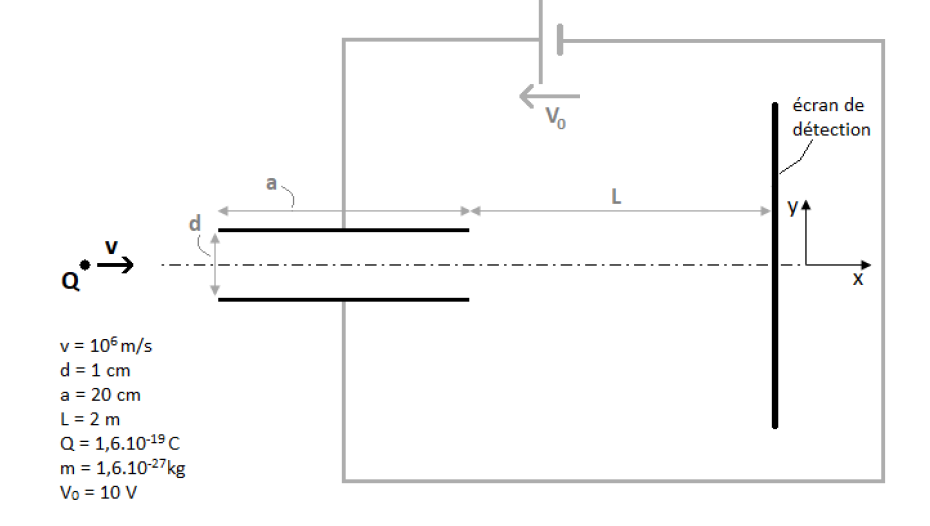
\includegraphics[width = 17cm]{TpQEx_Champs/Q1_TheoChampsJanv2019.PNG}
    %\caption{}
    \label{fig:Q1_TheoChampsJanv2019}
\end{figure}

\Question{
\newline
Calculer la position de détection y sur l’écran de détection en fonction des paramètres du système. Donner également sa valeur numérique. Utiliser le système d’axe donné sur le schéma (y positif vers le haut, avec l’origine au centre de l’écran de détection). \\\textbf{Négliger les effets de bords.}
}
{%C
}
\newpage
\subsection{Examen Janvier 2018 (Q1)}
Soit une spire circulaire de rayon R parcourue par un courant I. Soit une autre spire carrée ouverte de côté a. Les 2 spires sont éloignées d’une distance D l’une de l’autre et sont parallèles entre elles. \\
La situation est illustrée ci-dessous.
\begin{figure}[h!]
    \centering
    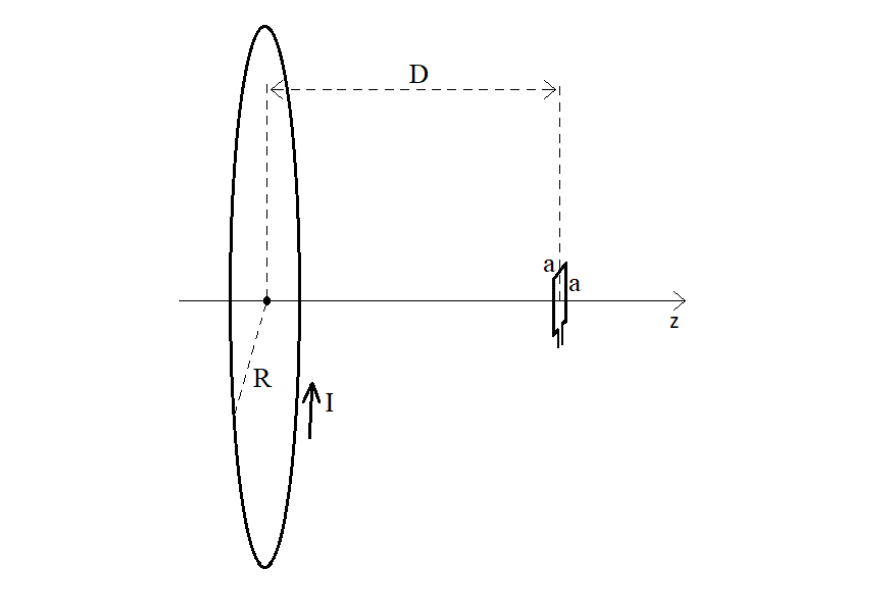
\includegraphics[width = 15cm]{TpQEx_Champs/Q1_TheoChampsJanv2018.PNG}
    %\caption{}
    \label{fig:Q1_TheoChampsJanv2018}
\end{figure}

\begin{enumerate}
    \item Calculer le champ magnétique ~B le long de l’axe z.
    \item Supposant la valeur de B constante sur la petite spire carrée (égale à la valeur au centre de la spire), calculer le flux capté par cette spire carrée ainsi que le coefficient d’inductance mutuelle entre les 2 spires.
    \item Calculer la tension induite e(t) induite sur la spire carrée si celle-ci se déplace à une vitesse constante v en direction de la spire circulaire. Supposer toujours que la valeur de B est constante sur la spire.
\end{enumerate}

\newpage
\subsection{Examen Janvier 2016 (Q2)}
Soit une sphère de rayon a. Cette sphère est constituée de 2 demi-sphères uniformément chargées d’une charge +Q et -Q. La situation est représentée ci-dessous. Le milieu dans lequel se trouve la sphère est le vide.\\
La situation est illustrée ci-dessous.
\begin{figure}[h!]
    \centering
    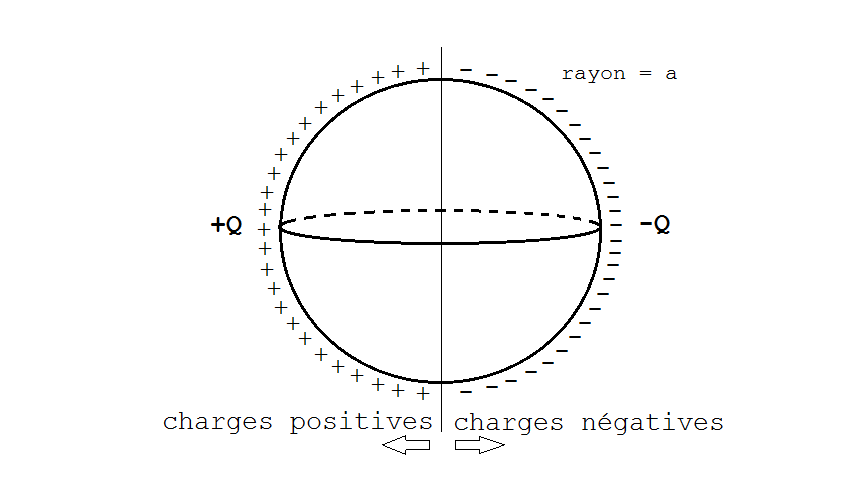
\includegraphics[width = 14cm]{TpQEx_Champs/Q2_TheoChampsJuin2016.PNG}
    %\caption{}
    \label{fig:Q2_TheoChampsJuin2016}
\end{figure}
Pour rappel :
\begin{figure}[h!]
    \centering
    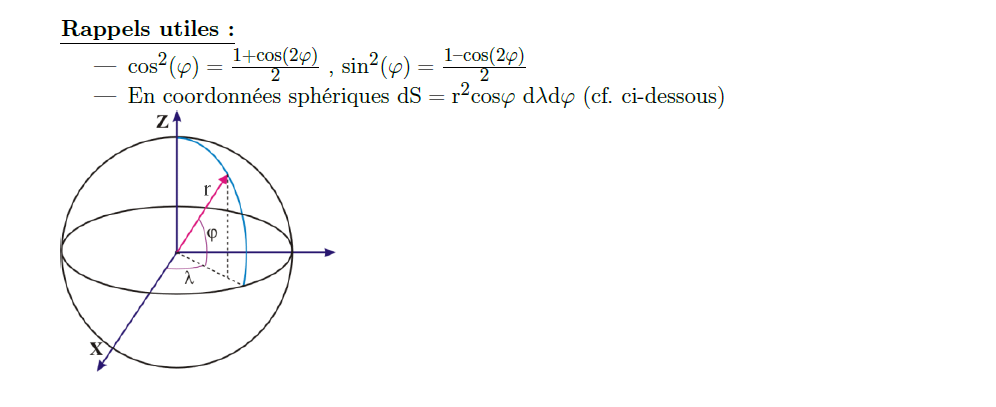
\includegraphics[width = 18cm]{TpQEx_Champs/Q2_Hint_TheoChampsJuin2016.PNG}
    %\caption{}
    \label{fig:Q2_Hint_TheoChampsJuin2016}
\end{figure}

\begin{enumerate}
    \item Le problème présente-t-il une symétrie sphérique ? Justifier.
    \item Est-ce que la sphère est parfaitement conductrice ? Justifier.
    \item Calculer la densité surfacique de charge $\sigma$ de chaque côté de la sphère.
    \item Que vaut le potentiel électrique V au centre de la sphère ? Justifier.
    \item Que vaut le champ électrique ~E au centre de la sphère ? Donner son amplitude, sa direction et son sens.
\end{enumerate}

\newpage
\subsection{Examen Septembre 2018 (Q2)}
Soient 2 fils chargés uniformément, l’un d’une densité linéique de charge $\rho$ et l’autre d’une densité $-\rho$ ($\rho > 0$). Les fils sont séparés par une distance d (entre leur centres), leur rayon est égal à a et ils sont de longueur infinie. Le système est plongé dans un milieu assimilable au vide. 
Le matériau des fils est un métal parfait.
\begin{figure}[h!]
    \centering
    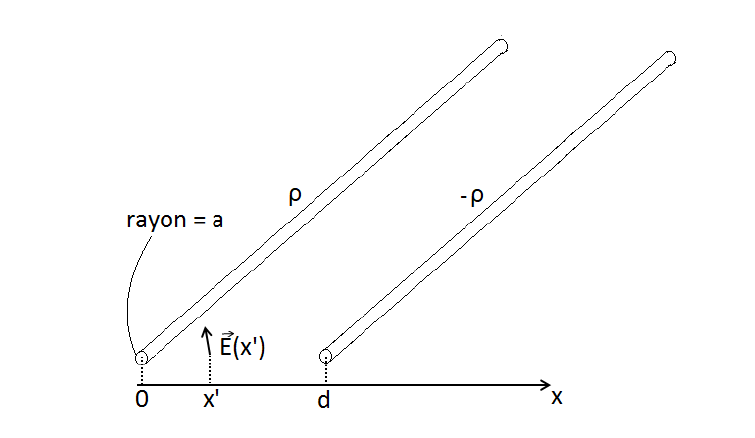
\includegraphics[width = 15cm]{TpQEx_Champs/Q2_TheoChampsSept2018.PNG}
    %\caption{}
    \label{fig:Q2_TheoChampsSept2018}
\end{figure}

\begin{enumerate}
    \item Calculer le champ électrique E existant entre les 2 conducteurs en fonction de $\rho$, d, a et x’. Supposer que $d \gg a$.
    \item Représenter qualitativement 3 lignes de champs électriques différentes sur le dessin ci-dessous. Représenter également la répartition des charges dans les 2 fils (via des "+" et des "-"). Les fils sont représentés par une vue en coupe, ils sont donc perpendiculaires à cette feuille.\\
    
    Que vaut le champ électrique à l’intérieur des fils ? 
    \begin{figure}[h!]
        \centering
        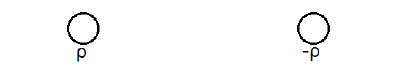
\includegraphics[width = 10cm]{TpQEx_Champs/Q2_Hint_TheoChampsSept2018.PNG}
        %\caption{}
        \label{fig:Q2_Hint_TheoChampsSept2018}
    \end{figure}
    \item Calculer la capacité par unité de longueur constituée par les 2 fils conducteurs.
\end{enumerate}

\newpage

\subsection{Examen Janvier 2020 (Q4)}

On considère le circuit magnétique suivant, constitué d’un matériau magnétique linéaire de perméabilité $µ_r$. 
\begin{figure}[h!]
    \centering
    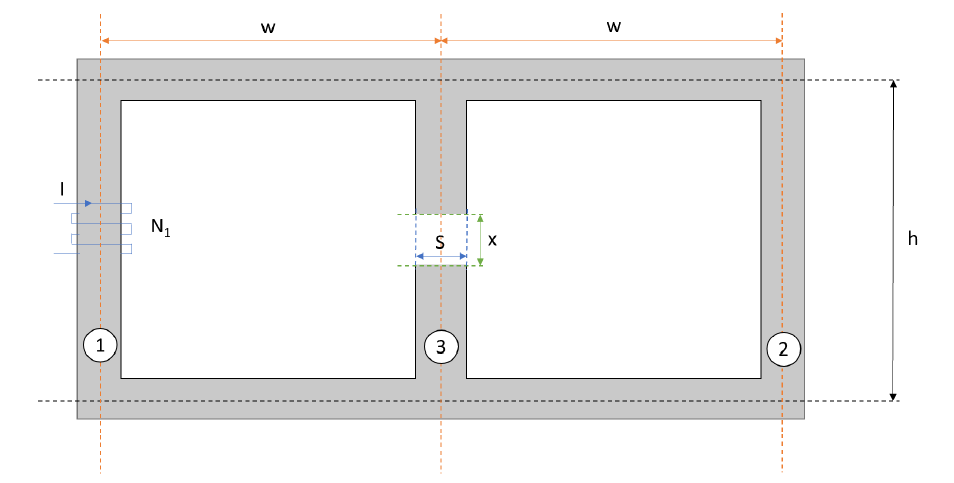
\includegraphics[width = 14cm]{TpQEx_Champs/Q4_TheoChampsJanv2020.PNG}
    %\caption{}
    \label{fig:Q4_TheoChampsJanv2020}
\end{figure}
Avec les hypothèses et caractéristiques suivantes :
\begin{figure}[h!]
    \centering
    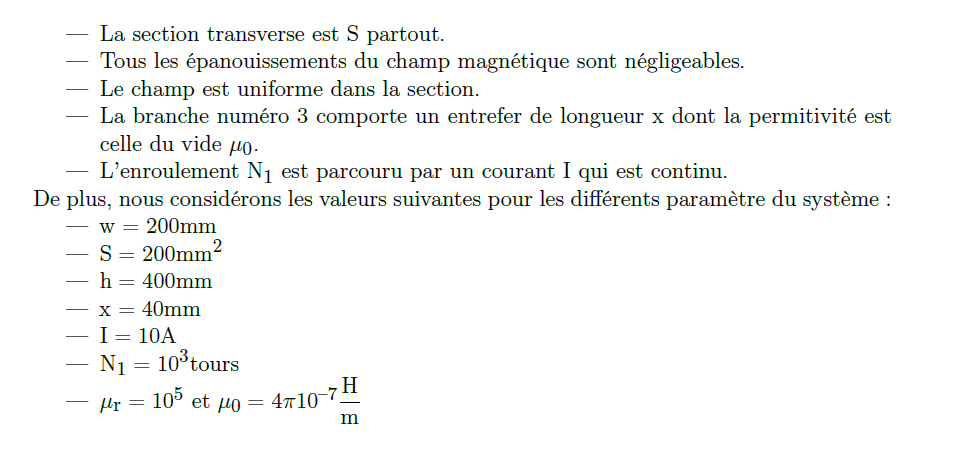
\includegraphics[width = 13cm]{TpQEx_Champs/Q4_Caracts_TheoChampsJanv2020.PNG}
    %\caption{}
    \label{fig:Q4_Caracts_TheoChampsJanv2020}
\end{figure}

\begin{enumerate}
    \item Calculez les réluctances des trois branches du circuit magnétique.
    \item Représentez le circuit électrique équivalent et déterminez le flux dans chaque branche du circuit magnétique.
\end{enumerate}

\newpage
\subsection{Examen Janvier 2017 (Q2)}

Soit le circuit à réluctances ci-dessous :
\begin{figure}[h!]
    \centering
    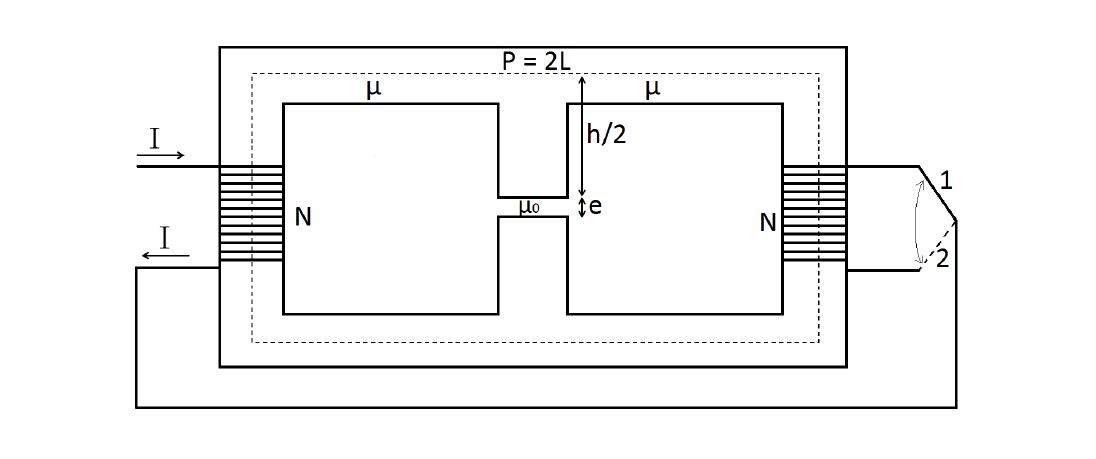
\includegraphics[width = 14cm]{TpQEx_Champs/Q2_TheoChampsJanv2017.PNG}
    %\caption{}
    \label{fig:Q2_TheoChampsJanv2017}
\end{figure}
Les données du système sont les suivantes :
\begin{figure}[h!]
    \centering
    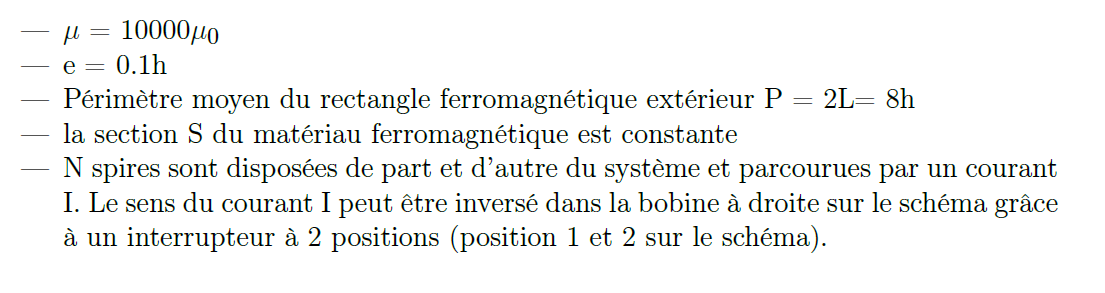
\includegraphics[width = 13cm]{TpQEx_Champs/Q2_Hint_TheoChampsJanv2017.PNG}
    %\caption{}
    \label{fig:Q2_Hint_TheoChampsJanv2017}
\end{figure}

\begin{enumerate}
    \item Calculer la réluctance du demi-périmètre de longueur L. Calculer également les 2 réluctances de la branche centrale (dans le matériau et dans
    l’air). Quelle réluctance est la plus grande ? Calculer le rapport entre la plus grande réluctance et les 2 autres.
    \item Pour les 2 positions de l’interrupteur, représenter le circuit électrique équivalent à ce circuit magnétique. Attention à bien définir tous
    les éléments et grandeurs du circuit ainsi que la position de l’interrupteur correspondant à chaque circuit.
    \item Pour les 2 positions de l’interrupteur, calculer le flux circulant dans le périmètre P du matériau ferromagnétique. Vous pouvez faire des hypothèses simplificatrices pour le calcul.
\end{enumerate}
\end{document}
%% fancy header & foot
\pagestyle{fancy}
\lhead{[ELEC-H-2001] Électricité\\ Séance \no 10 : Séance récapitulative - Théorie des circuits \ifthenelse{\boolean{corrige}}{~-- corrigé}{}}
\rhead{v1.0.0\\ page \thepage}
\cfoot{}
%%

\pdfinfo{
/Author (Renaud Theunissen et Youssef Agram, ULB -- BEAMS-EE)
/Title (Séance 10 ELEC-H-2001, Séance récapitulative - Théorie des circuits)
/ModDate (D:\pdfdate)
}

\hypersetup{
pdftitle={Séance 10 [ELEC-H-2001] Électricité : Séance 11 ELEC-H-2001, Séance récapitulative - Théorie des circuits},
pdfauthor={Renaud Theunissen et Youssef Agram, ©2020 ULB - BEAMS-EE},}

\setlength{\parskip}{0.5cm plus4mm minus3mm} %espacement entre §
\setlength{\parindent}{0pt}


\begin{document}
\long\def\nothx/*#1*/{}
\tptitle{}{Séance 10~: Séance récapitulative - Théorie des circuits}
\section{But de la séance}
L'objectif de cette séance est de vous proposer des questions pratique typiques d'examen pour la partie théorie des circuits.
Cette séance sert de synthèse aux séances d'exercices consacrées aux circuits.

\section{Pré-requis}
Avant la séance, vous aurez relu les chapitres et sections suivants:
\begin{itemize}
	\item Chapitre 1 - Circuits à éléments concentrés
		\begin{itemize}
		\item Section 1.6 - Puissance instantanée, conventions et passivité
		\end{itemize}
	\item Chapitre 2 - Dipôles idéaux
	    \begin{itemize}
	        \item Section 2.2 - Dipôles réels >< Dipôles idéaux
	        \item Section 2.3 - Charges idéales : trois effets physiques
	        \item Section 2.6 - Sources idéales
	    \end{itemize}
	\item Chapitre 4 - Équivalence de Thévenin et adaptation d'impédance
		\begin{itemize}
		\item Section 4.1 - Circuits équivalents et théorèmes de Thévenin et Norton
		\item Section 4.2 - Impédance d'entrée, impédance de sortie (et fem à vide)
		\item Section 4.3 - Adaptation d'impédance
		\end{itemize}
	\item Chapitre 5 - Résoudre un circuit : procédure de base et accélérateurs
	    \begin{itemize}
	        \item Section 5.1 - Vocabulaire lié aux circuits 
	        \item Section 5.2 - Lois de Kirchhoff
	        \item Section 5.3 - Procédure canonique en 6 étapes
	        \item Section 5.4 - Illustration : Diviseur résistif (étendu aux impédances)
	        \item Section 5.5 - Équivalences série et parallèle
	        \item Section 5.6 - Utilisation des théorèmes de Thévenin et Norton pour résoudre un circuit
	        \item Section 5.8 - Théorème de superposition
	    \end{itemize}
	\item Chapitre 6 - Résoudre un circuit réactif dans le domaine temporel
	    \begin{itemize}
	        \item Section 6.1 - Éléments réactifs : Rappels 
		    \item Section 6.2 - Analyse temporelle du circuit RC (source en échelons)
		    \item Section 6.3 - Analyse temporelle du circuit RL (source en échelons)
		    \item Section 6.5 - Analyse temporelle du circuit RL (source sinusoïdale avec échelon)
		    \item Section 6.6 - Analyse temporelle du circuit RLC
	    \end{itemize}
	\item Chapitre 7 - Résoudre un circuit réactif dans le domaine fréquentiel
	    \begin{itemize}
	        \item Section 7.3 - Phaseurs
		    \item Section 7.4 - Impédances et admittances
	    \end{itemize}
\end{itemize}

\vspace{5pt}

\newpage

\section{Théorie des circuits - Exercices d'examens}
\subsection{Examen Juin 2016 (Q4)}

Soit le circuit suivant \\

\begin{figure}[h!]
    \centering
    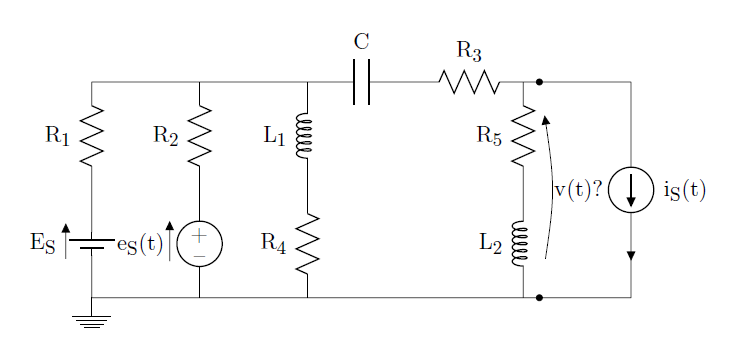
\includegraphics[width = 17cm]{TpQEx_Circuits/Q4_Juin_2016.PNG}
    %\caption{}
    \label{fig:Q4_TheoCircuitsJuin2016}
\end{figure}
Où les sources sont $E_S = E_1$, $e_{S}(t) = E_1 +E_2*sin(\omega_1 t)$ et $i_s(t) = I * (1+cos(\omega_2 t+\Phi)$. 
Les valeurs des différents paramètres sont les suivantes :
\begin{figure}[h!]
    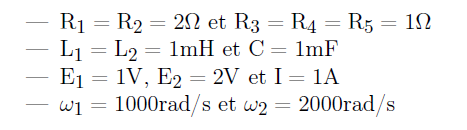
\includegraphics[width = 10cm]{TpQEx_Circuits/Q4_Juin_2016_HINT.PNG}
    %\caption{}
    \label{fig:Q4_TheoCircuitsJuin2016_HINT}
\end{figure}

\Question{
\newline
On vous demande de déterminer la tension v(t) en suivant les indications suivantes :
\begin{enumerate}
    \item Suivez la procédure canonique
    \item Expliquez votre démarche et mettez en évidence les étapes qui vous sont nécessaires pour trouver les résultats intermédiaires
    \item Utilisez au minimum une fois un équivalent de Thévenin en expliquant en quoi cette méthode vous permet de faciliter la résolution de ce circuit
    \item Vous ne devez pas développer les racines et arctangentes jusqu’au bout. Par exemple, si vous tombez sur $\sqrt{7^2+11^2}$ ou $Arg(7+11j)$, notez respectivement $\sqrt{170}$ ou $arctg(\dfrac{11}{7})$ (pas de valeurs avec décimales)
\end{enumerate}
}
{En utilisant le théorème de superposition\\
$E_S$ : la capa se comporte comme un circuit ouvert –> $V_1 = 0V$\\
\textbf{Composante continue} de $e_s(t)$ : Idem –> $V_2 = 0V$\\
\textbf{Composante continue} de $i_S(t)$ : $V_3$ = $- R_5 * I = – 1V$\\
$E_2sin(\omega_1t)$ : Thévenin
\begin{equation*}
    Z_1 = R_1 (R_4+j\omega_1L_1) \implies Z_1 = \dfrac{2+2j}{3+j}
\end{equation*}
\begin{equation*}
    Z_2=R_3+\dfrac{1}{j\omega_1C} \implies Z_2 = 1–j
\end{equation*}
\begin{equation*}
    Z_3 = R_5+j\omega_1L_2 \implies Z_3=1+j
\end{equation*}
\begin{equation*}
    Z_{Th} = Z_2 + R_2
\end{equation*}
\begin{equation*}
    Z_1 = 1 – j + \dfrac{1+j}{2+j} \implies Z_1 = \dfrac{4}{2+j}
\end{equation*}
\begin{equation*}
    \underline{V}_{Th} = \dfrac{Z_1}{R_2+Z_1} \underline{E}_S \implies \underline{V}_{Th}= \dfrac{1+j}{4+2j}\underline{E}_S
\end{equation*}
\begin{equation*}
    \underline{V}_4 = \dfrac{Z_3}{Z_3+Z_{Th}} \implies \underline{V}_4=\dfrac{-1+2j}{7+11j}\underline{E}_S
\end{equation*}
\begin{equation*}
    v_4(t) = \dfrac{2\sqrt{5}}{\sqrt{170}}sin(1000t - arctan(2)-acrtan\left(\dfrac{11}{7}\right)
\end{equation*}

$I*cos(\omega_2t + \Phi)$ : Thévenin
\begin{equation*}
    Z_A = R_1//R_2//(R_4 + j\omega_4*L_1) = \dfrac{1+2j}{2+2j}
\end{equation*}
\begin{equation*}
    Z_B = R_3 + \dfrac{1}{j\omega_2*C}=1-0,5j
\end{equation*}
\begin{equation*}
    Z_3= R_5 +j\omega_2*L_2 = 1+2j
\end{equation*}
\begin{equation*}
    Z_{eq} = (Z_A + Z_B)//Z_3 = \dfrac{-2+11j}{2+9j}
\end{equation*}
\begin{equation*}
    \underline{V}_5 = -Z_{eq}*\underline{I}_S = \dfrac{2-11j}{2+9j}*e^{\Phi} 
\end{equation*}
\begin{equation*}
    \underline{V}_{5} = \dfrac{5*\sqrt{5}}{\sqrt{85}}*e^{j*\left(\Phi + arctan(\dfrac{11}{2}) - arctan(\dfrac{9}{2})\right)}
\end{equation*}
\begin{equation*}
    v_5(t) = \dfrac{5*\sqrt{5}}{\sqrt{85}}*cos\left(2000*t+\Phi+ arctan(\dfrac{11}{2}) - arctan(\dfrac{9}{2})\right)
\end{equation*}

On trouve ainsi\\
\begin{equation*}
    v(t) = V_1 + V_2 + V_3 + v_4(t) + v_5(t)

    v(t) = –1 + \dfrac{2}{\sqrt{170}}*sin\left(1000*t - arctan(\dfrac{11}{7})\right) - \dfrac{\sqrt{125}}{\sqrt{80}}*cos\left(2000*t+\Phi-arctan(2) - arctan(\dfrac{3}{2})\right)
\end{equation*}

}

\newpage
\subsection{Examen Janvier 2014 (Q3)}
Soit le circuit suivant :

\begin{figure}[h!]
    \centering
    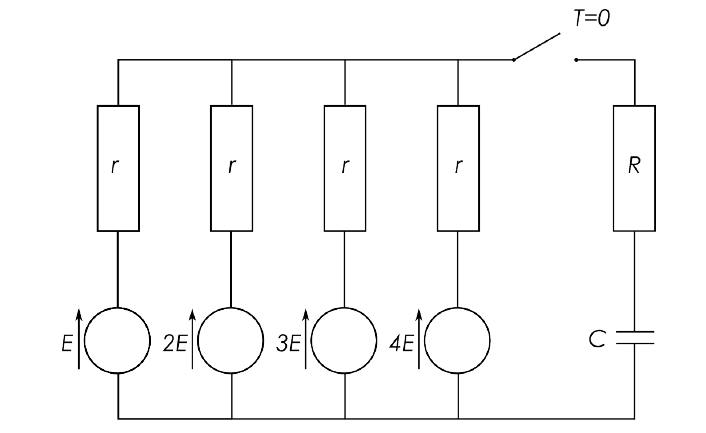
\includegraphics[width = 11cm]{TpQEx_Circuits/Q3_Janv_2014.PNG}
    %\caption{}
    \label{fig:Q3_TheoCircuitsJanv2014}
\end{figure}
Où $E = 20V$, $r = 4\Omega$,$R = 1\Omega$ et $C = 0,1 F$.
Avant $t = 0$, l'interrupteur est ouvert. On ferme l'interrupteur à l'instant $t = 0$. La charge initiale de la capacité est nulle.
Après une prise de mesure, on a relevé les deux courbes suivantes (temps [s] en abscisse et courant [A] ou tension [V] en ordonnée).
\begin{figure}[h!!]
    \centering
    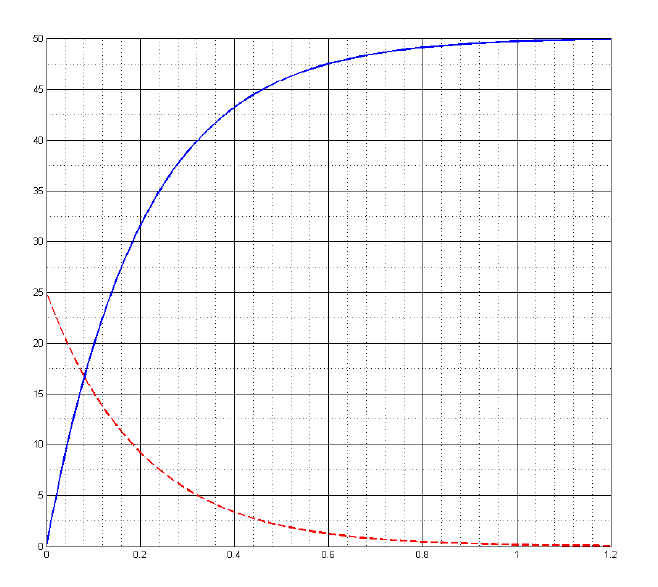
\includegraphics[width = 12cm]{TpQEx_Circuits/Q3_Janv_2014_Graph.PNG}
    %\caption{}
    \label{fig:Q3_TheoCircuitsJanv2014_Graph}
\end{figure}

\begin{itemize}
    \item \Question{Identifiez l’élément du schéma (source(s), capacité, resistance(s)) auquel se rapportent ces deux graphes.
    }
    {
    Ici l'élément dont il est question est un condensateur.
    }
    \item \Question{Identifiez la grandeur (tension(s) ou courant(s)) présente sur l’ordonnée pour chaque courbe (trait continu et trait discontinu).
    }
    {
    \textbf{Trait continu} :\\
    Cette courbe représente la tensions aux bornes du condensateur $v_C(t)$.\\
    \textbf{Trait discontinu} :\\
    Cette courbe re présente l'intensité du courant traversant le condensateur $i_C(t)$.
    }
    \item \Question{Sur base de ce graphique, déterminer la valeur de la constante de temps $\tau$ du circuit.
    }
    {
    La constante de temps $\tau$ est par définition le temps nécessaire à la tension aux bornes du condensateur pour atteindre 63\% de sa valeur de régime :
    \begin{equation*}
        v_C(\tau) = v_C(\infty) *(1-\exp{-1})\approx 0,63*v_C(\infty)
    \end{equation*}
    Graphiquement, il suffit de tracer une ligne horizontale passant par $0,63*50 = 31,5V$.\\
    L'intersection avec le graphique de $v_C(t)$ donne $\tau = 0,2s$.
    }
    \newpage\item \Question{Déterminez les paramètres $R_{th}$ et $V_{th}$ de l’équivalent de Thévenin du circuit vu aux bornes du condensateur.
    }
    {
    \begin{itemize}
        \item Pour $R_{Th}$ :\\
        Pour trouver la résistance équivalente de Thévenin, il faut court-circuiter les sources du circuit.
        Par les propriétés de la mise en parallèle et de la mise en série des résistances on trouve : 
        \begin{equation*}
            R_{Th} = R + (r//r//r//r)\implies R_{Th}=R+\dfrac{r}{4}
        \end{equation*}
        \begin{figure}[h!!!]
            \centering
            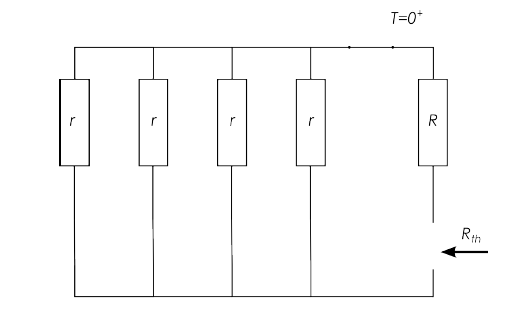
\includegraphics[width = 10cm]{TpQEx_Circuits/TP11Q2_Reso1.PNG}
    %\caption{}
            \label{fig:Q3_TheoCircuitsJanv2014_Reso1}
        \end{figure}
        \item Pour $V_{Th}$ :\\
        Pour trouver la tension équivalente de Thévenin, on doit résoudre le circuit à vide (remplacer le condensateur par un circuit ouvert). Le courant passant par la branche de droite sera alors nul et il n'y a pas de chute de potentiel dans la résistance $R$ (car $V_R = R*i = 0$).
        \begin{figure}[h!!!!]
            \centering
            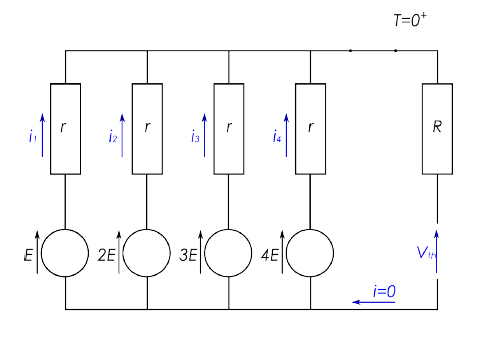
\includegraphics[width = 10cm]{TpQEx_Circuits/TP11Q2_Reso2.PNG}
    %\caption{}
            \label{fig:Q3_TheoCircuitsJanv2014_Reso2}
        \end{figure}
        \item \textbf{Résolution 1 - Lois de Kirchhoff}\\
        Soit $i_k(t)$ le courant passant dans la $k^{ième}$ branche (de gauche à droite).
        La mise en parallèle des cinq branches nous permet d'égaler les tensions :
        \begin{equation*}
            V_{Th} = E - r_{i_1} = 2E - r_{i_2} = 3E - r_{i_3} = 4E - r_{i_4}
        \end{equation*}
        Par la loi des noeuds, on a donc :
        \begin{equation*}
            i(t) = \sum^4_{k=1}\left(i_k(t)\right) = 0
            
            \iff i_1+i_1+\dfrac{E}{r}+i_1\dfrac{2E}{r}+i_1\dfrac{3E}{r} = 4i_1+6\dfrac{E}{r} = 0
            
            \iff i_1 = \dfrac{-3}{2}\dfrac{E}{r}
            
        \end{equation*}
        Et donc finalement : $V_{Th}=E-r*i_1 = \dfrac{5}{2}*E$
        \item \textbf{Résolution 2 - Théorème de superposition}\\
        Soit $E_i(i = 1,2,3,4)$ les 4 sources et $V_{Th_i}$les contributions de chacune d'elle à la tension de Thévenin.\\
        On annule donc toutes les sources sauf $E_i$ pour les 4 cas (i=1,2,3,4), on calcule chacune des contributions puis on les somme pour avoir $V_{Th}$.\\
        \textit{Remarque}\\
        Beaucoup d'entre vous 
    \end{itemize}
    }
\end{itemize}

\newpage
\subsection{Examen Janvier 2015 (Q1.3)}
Soit le circuit suivant avec :
\begin{itemize}
    \item $E_S$ une source de tension continue d'amplitude $E$
    \item 7 résistances de même valeur $R$
    \item Un condensateur $C$
\end{itemize}
\begin{figure}[h!]
    \centering
    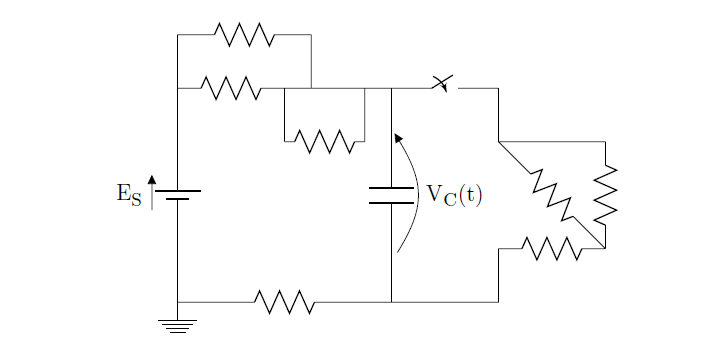
\includegraphics[width = 14cm]{TpQEx_Circuits/Q1_3_Janv_2015.PNG}
    %\caption{}
    \label{fig:Q1_3_TheoCircuits_Janv2015}
\end{figure}
On ferme l'interrupteur à l'instant $t=0$.\\
Quelle est l'expression analytique de $V_C(t)$ pour tout temps $t$?


\newpage
\subsection{Examen Septembre 2015 (Q4)}

\begin{figure}[h!]
    \centering
    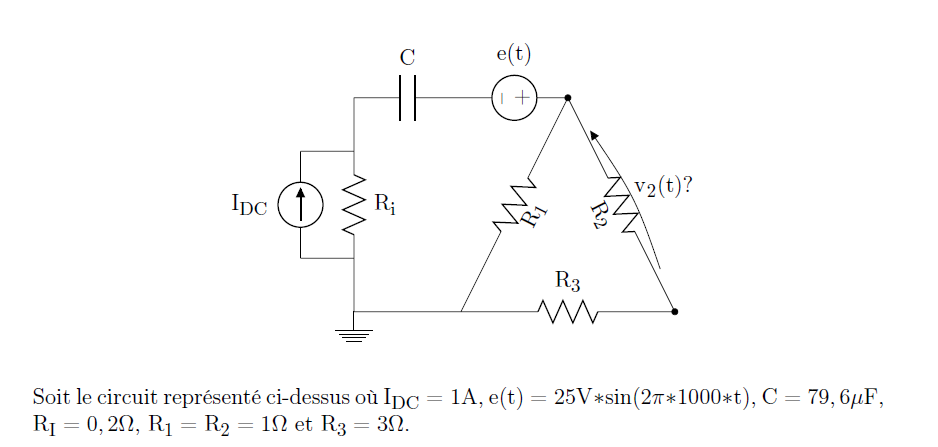
\includegraphics[width = 17cm]{TpQEx_Circuits/Q4_Sept_2015.PNG}
    %\caption{}
    \label{fig:Q4_TheoCircuitsSept2015}
\end{figure}
Que vaut $V_2$, l'amplitude de $v_2(t)$ pour tout temps $t$?

\newpage

\subsection{Examen Septembre 2019 (Q1) Modifiée}

\begin{figure}[h!]
    \centering
    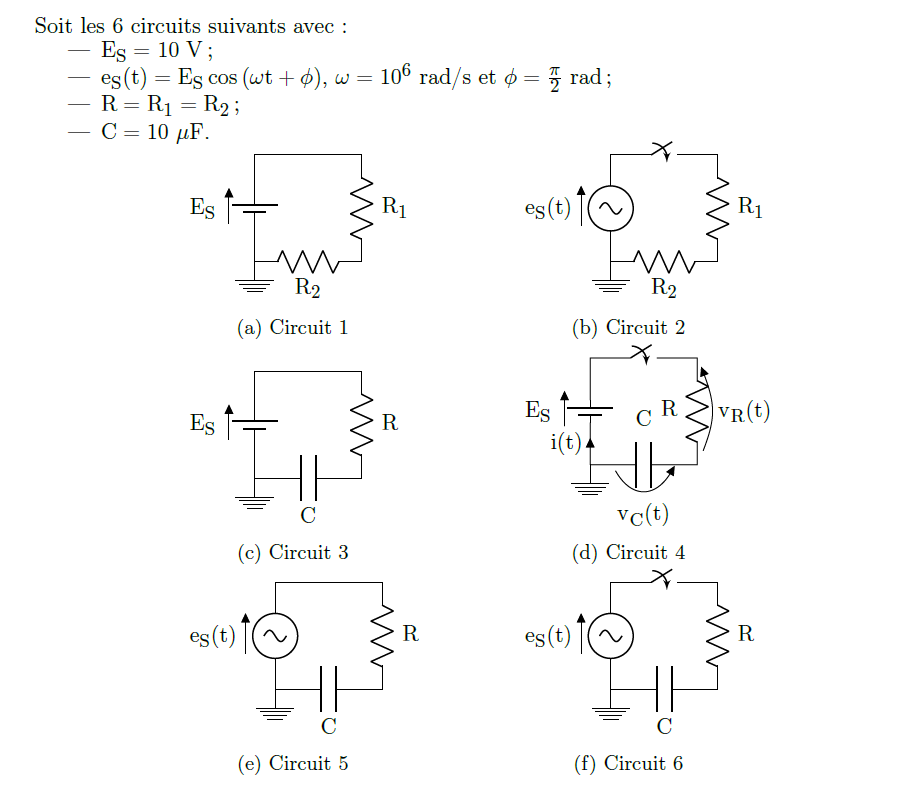
\includegraphics[width = 17cm]{TpQEx_Circuits/Q1_Sept_2019.PNG}
    %\caption{}
    \label{fig:Q1_TheoCircuitsSept2019}
\end{figure}


\begin{enumerate}
    \item Pour quels circuits devrions-nous utiliser les phaseurs \textbf{uniquement} pour résoudre le circuit?
    \item Pour quels circuits devrions-nous utiliser les lois long terme \textbf{uniquement} pour résoudre le circuit?
    \item Pour quels circuits la méthode des phaseurs ne suffira pas à résoudre le circuit?
    \item Déterminez la tension aux bornes du condensateur pour les circuits 3 à 6 et pour tout temps.
    \item Déterminez la tension aux bornes de la résistance $R_1$ des circuits 1 et 2, pour tous temps t
\end{enumerate}

\newpage
\subsection{Examen Septembre 2019 (Q2)}

Soit le circuit suivant comportant :
\begin{itemize}
    \item Une source de tension sinusoïdale : $e_1(t) = E_1 sin(\omega t)$
    \item Une deuxième source de tension sinusoïdale : $e_2(t) = E_2 sin(\omega t+\alpha)$
    \item Une source de courant continu : $I_S$
    \item 4 résistances de même valeur : $R_1$,$R_2$,$R_3$ et $R_4$
    \item Un condensateur $C$ et une inductance $L$
\end{itemize}
\begin{figure}[h!]
    \centering
    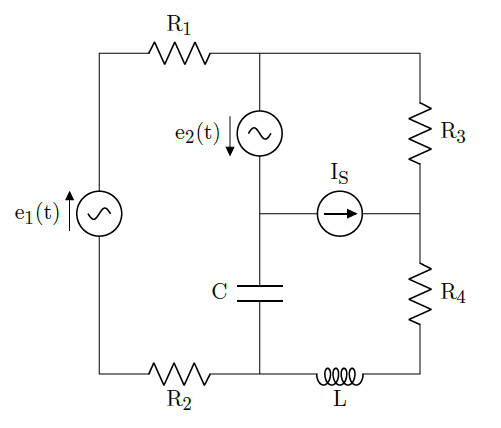
\includegraphics[width = 14cm]{TpQEx_Circuits/Q2_Sept_2019.PNG}
    %\caption{}
    \label{fig:Q2_TheoCircuitsSept2019}
\end{figure}

En utilisant les principes et théorèmes vus au cours, déterminez l'équivalent de Thévenin de ce circuit vu par la résistance $R_4$ de la manière la plus efficace possible.
\end{document}